\documentclass[11pt]{article}

    \usepackage[breakable]{tcolorbox}
    \usepackage{parskip} % Stop auto-indenting (to mimic markdown behaviour)
    
    \usepackage{iftex}
    \ifPDFTeX
    	\usepackage[T1]{fontenc}
    	\usepackage{mathpazo}
    \else
    	\usepackage{fontspec}
    \fi

    % Basic figure setup, for now with no caption control since it's done
    % automatically by Pandoc (which extracts ![](path) syntax from Markdown).
    \usepackage{graphicx}
    % Maintain compatibility with old templates. Remove in nbconvert 6.0
    \let\Oldincludegraphics\includegraphics
    % Ensure that by default, figures have no caption (until we provide a
    % proper Figure object with a Caption API and a way to capture that
    % in the conversion process - todo).
    \usepackage{caption}
    \DeclareCaptionFormat{nocaption}{}
    \captionsetup{format=nocaption,aboveskip=0pt,belowskip=0pt}

    \usepackage[Export]{adjustbox} % Used to constrain images to a maximum size
    \adjustboxset{max size={0.9\linewidth}{0.9\paperheight}}
    \usepackage{float}
    \floatplacement{figure}{H} % forces figures to be placed at the correct location
    \usepackage{xcolor} % Allow colors to be defined
    \usepackage{enumerate} % Needed for markdown enumerations to work
    \usepackage{geometry} % Used to adjust the document margins
    \usepackage{amsmath} % Equations
    \usepackage{amssymb} % Equations
    \usepackage{textcomp} % defines textquotesingle
    % Hack from http://tex.stackexchange.com/a/47451/13684:
    \AtBeginDocument{%
        \def\PYZsq{\textquotesingle}% Upright quotes in Pygmentized code
    }
    \usepackage{upquote} % Upright quotes for verbatim code
    \usepackage{eurosym} % defines \euro
    \usepackage[mathletters]{ucs} % Extended unicode (utf-8) support
    \usepackage{fancyvrb} % verbatim replacement that allows latex
    \usepackage{grffile} % extends the file name processing of package graphics 
                         % to support a larger range
    \makeatletter % fix for grffile with XeLaTeX
    \def\Gread@@xetex#1{%
      \IfFileExists{"\Gin@base".bb}%
      {\Gread@eps{\Gin@base.bb}}%
      {\Gread@@xetex@aux#1}%
    }
    \makeatother

    % The hyperref package gives us a pdf with properly built
    % internal navigation ('pdf bookmarks' for the table of contents,
    % internal cross-reference links, web links for URLs, etc.)
    \usepackage{hyperref}
    % The default LaTeX title has an obnoxious amount of whitespace. By default,
    % titling removes some of it. It also provides customization options.
    \usepackage{titling}
    \usepackage{longtable} % longtable support required by pandoc >1.10
    \usepackage{booktabs}  % table support for pandoc > 1.12.2
    \usepackage[inline]{enumitem} % IRkernel/repr support (it uses the enumerate* environment)
    \usepackage[normalem]{ulem} % ulem is needed to support strikethroughs (\sout)
                                % normalem makes italics be italics, not underlines
    \usepackage{mathrsfs}
    

    
    % Colors for the hyperref package
    \definecolor{urlcolor}{rgb}{0,.145,.698}
    \definecolor{linkcolor}{rgb}{.71,0.21,0.01}
    \definecolor{citecolor}{rgb}{.12,.54,.11}

    % ANSI colors
    \definecolor{ansi-black}{HTML}{3E424D}
    \definecolor{ansi-black-intense}{HTML}{282C36}
    \definecolor{ansi-red}{HTML}{E75C58}
    \definecolor{ansi-red-intense}{HTML}{B22B31}
    \definecolor{ansi-green}{HTML}{00A250}
    \definecolor{ansi-green-intense}{HTML}{007427}
    \definecolor{ansi-yellow}{HTML}{DDB62B}
    \definecolor{ansi-yellow-intense}{HTML}{B27D12}
    \definecolor{ansi-blue}{HTML}{208FFB}
    \definecolor{ansi-blue-intense}{HTML}{0065CA}
    \definecolor{ansi-magenta}{HTML}{D160C4}
    \definecolor{ansi-magenta-intense}{HTML}{A03196}
    \definecolor{ansi-cyan}{HTML}{60C6C8}
    \definecolor{ansi-cyan-intense}{HTML}{258F8F}
    \definecolor{ansi-white}{HTML}{C5C1B4}
    \definecolor{ansi-white-intense}{HTML}{A1A6B2}
    \definecolor{ansi-default-inverse-fg}{HTML}{FFFFFF}
    \definecolor{ansi-default-inverse-bg}{HTML}{000000}

    % commands and environments needed by pandoc snippets
    % extracted from the output of `pandoc -s`
    \providecommand{\tightlist}{%
      \setlength{\itemsep}{0pt}\setlength{\parskip}{0pt}}
    \DefineVerbatimEnvironment{Highlighting}{Verbatim}{commandchars=\\\{\}}
    % Add ',fontsize=\small' for more characters per line
    \newenvironment{Shaded}{}{}
    \newcommand{\KeywordTok}[1]{\textcolor[rgb]{0.00,0.44,0.13}{\textbf{{#1}}}}
    \newcommand{\DataTypeTok}[1]{\textcolor[rgb]{0.56,0.13,0.00}{{#1}}}
    \newcommand{\DecValTok}[1]{\textcolor[rgb]{0.25,0.63,0.44}{{#1}}}
    \newcommand{\BaseNTok}[1]{\textcolor[rgb]{0.25,0.63,0.44}{{#1}}}
    \newcommand{\FloatTok}[1]{\textcolor[rgb]{0.25,0.63,0.44}{{#1}}}
    \newcommand{\CharTok}[1]{\textcolor[rgb]{0.25,0.44,0.63}{{#1}}}
    \newcommand{\StringTok}[1]{\textcolor[rgb]{0.25,0.44,0.63}{{#1}}}
    \newcommand{\CommentTok}[1]{\textcolor[rgb]{0.38,0.63,0.69}{\textit{{#1}}}}
    \newcommand{\OtherTok}[1]{\textcolor[rgb]{0.00,0.44,0.13}{{#1}}}
    \newcommand{\AlertTok}[1]{\textcolor[rgb]{1.00,0.00,0.00}{\textbf{{#1}}}}
    \newcommand{\FunctionTok}[1]{\textcolor[rgb]{0.02,0.16,0.49}{{#1}}}
    \newcommand{\RegionMarkerTok}[1]{{#1}}
    \newcommand{\ErrorTok}[1]{\textcolor[rgb]{1.00,0.00,0.00}{\textbf{{#1}}}}
    \newcommand{\NormalTok}[1]{{#1}}
    
    % Additional commands for more recent versions of Pandoc
    \newcommand{\ConstantTok}[1]{\textcolor[rgb]{0.53,0.00,0.00}{{#1}}}
    \newcommand{\SpecialCharTok}[1]{\textcolor[rgb]{0.25,0.44,0.63}{{#1}}}
    \newcommand{\VerbatimStringTok}[1]{\textcolor[rgb]{0.25,0.44,0.63}{{#1}}}
    \newcommand{\SpecialStringTok}[1]{\textcolor[rgb]{0.73,0.40,0.53}{{#1}}}
    \newcommand{\ImportTok}[1]{{#1}}
    \newcommand{\DocumentationTok}[1]{\textcolor[rgb]{0.73,0.13,0.13}{\textit{{#1}}}}
    \newcommand{\AnnotationTok}[1]{\textcolor[rgb]{0.38,0.63,0.69}{\textbf{\textit{{#1}}}}}
    \newcommand{\CommentVarTok}[1]{\textcolor[rgb]{0.38,0.63,0.69}{\textbf{\textit{{#1}}}}}
    \newcommand{\VariableTok}[1]{\textcolor[rgb]{0.10,0.09,0.49}{{#1}}}
    \newcommand{\ControlFlowTok}[1]{\textcolor[rgb]{0.00,0.44,0.13}{\textbf{{#1}}}}
    \newcommand{\OperatorTok}[1]{\textcolor[rgb]{0.40,0.40,0.40}{{#1}}}
    \newcommand{\BuiltInTok}[1]{{#1}}
    \newcommand{\ExtensionTok}[1]{{#1}}
    \newcommand{\PreprocessorTok}[1]{\textcolor[rgb]{0.74,0.48,0.00}{{#1}}}
    \newcommand{\AttributeTok}[1]{\textcolor[rgb]{0.49,0.56,0.16}{{#1}}}
    \newcommand{\InformationTok}[1]{\textcolor[rgb]{0.38,0.63,0.69}{\textbf{\textit{{#1}}}}}
    \newcommand{\WarningTok}[1]{\textcolor[rgb]{0.38,0.63,0.69}{\textbf{\textit{{#1}}}}}
    
    
    % Define a nice break command that doesn't care if a line doesn't already
    % exist.
    \def\br{\hspace*{\fill} \\* }
    % Math Jax compatibility definitions
    \def\gt{>}
    \def\lt{<}
    \let\Oldtex\TeX
    \let\Oldlatex\LaTeX
    \renewcommand{\TeX}{\textrm{\Oldtex}}
    \renewcommand{\LaTeX}{\textrm{\Oldlatex}}
    % Document parameters
    % Document title
    \title{DEL\_Rechercheaufgabe}
    
    
    
    
    
% Pygments definitions
\makeatletter
\def\PY@reset{\let\PY@it=\relax \let\PY@bf=\relax%
    \let\PY@ul=\relax \let\PY@tc=\relax%
    \let\PY@bc=\relax \let\PY@ff=\relax}
\def\PY@tok#1{\csname PY@tok@#1\endcsname}
\def\PY@toks#1+{\ifx\relax#1\empty\else%
    \PY@tok{#1}\expandafter\PY@toks\fi}
\def\PY@do#1{\PY@bc{\PY@tc{\PY@ul{%
    \PY@it{\PY@bf{\PY@ff{#1}}}}}}}
\def\PY#1#2{\PY@reset\PY@toks#1+\relax+\PY@do{#2}}

\expandafter\def\csname PY@tok@w\endcsname{\def\PY@tc##1{\textcolor[rgb]{0.73,0.73,0.73}{##1}}}
\expandafter\def\csname PY@tok@c\endcsname{\let\PY@it=\textit\def\PY@tc##1{\textcolor[rgb]{0.25,0.50,0.50}{##1}}}
\expandafter\def\csname PY@tok@cp\endcsname{\def\PY@tc##1{\textcolor[rgb]{0.74,0.48,0.00}{##1}}}
\expandafter\def\csname PY@tok@k\endcsname{\let\PY@bf=\textbf\def\PY@tc##1{\textcolor[rgb]{0.00,0.50,0.00}{##1}}}
\expandafter\def\csname PY@tok@kp\endcsname{\def\PY@tc##1{\textcolor[rgb]{0.00,0.50,0.00}{##1}}}
\expandafter\def\csname PY@tok@kt\endcsname{\def\PY@tc##1{\textcolor[rgb]{0.69,0.00,0.25}{##1}}}
\expandafter\def\csname PY@tok@o\endcsname{\def\PY@tc##1{\textcolor[rgb]{0.40,0.40,0.40}{##1}}}
\expandafter\def\csname PY@tok@ow\endcsname{\let\PY@bf=\textbf\def\PY@tc##1{\textcolor[rgb]{0.67,0.13,1.00}{##1}}}
\expandafter\def\csname PY@tok@nb\endcsname{\def\PY@tc##1{\textcolor[rgb]{0.00,0.50,0.00}{##1}}}
\expandafter\def\csname PY@tok@nf\endcsname{\def\PY@tc##1{\textcolor[rgb]{0.00,0.00,1.00}{##1}}}
\expandafter\def\csname PY@tok@nc\endcsname{\let\PY@bf=\textbf\def\PY@tc##1{\textcolor[rgb]{0.00,0.00,1.00}{##1}}}
\expandafter\def\csname PY@tok@nn\endcsname{\let\PY@bf=\textbf\def\PY@tc##1{\textcolor[rgb]{0.00,0.00,1.00}{##1}}}
\expandafter\def\csname PY@tok@ne\endcsname{\let\PY@bf=\textbf\def\PY@tc##1{\textcolor[rgb]{0.82,0.25,0.23}{##1}}}
\expandafter\def\csname PY@tok@nv\endcsname{\def\PY@tc##1{\textcolor[rgb]{0.10,0.09,0.49}{##1}}}
\expandafter\def\csname PY@tok@no\endcsname{\def\PY@tc##1{\textcolor[rgb]{0.53,0.00,0.00}{##1}}}
\expandafter\def\csname PY@tok@nl\endcsname{\def\PY@tc##1{\textcolor[rgb]{0.63,0.63,0.00}{##1}}}
\expandafter\def\csname PY@tok@ni\endcsname{\let\PY@bf=\textbf\def\PY@tc##1{\textcolor[rgb]{0.60,0.60,0.60}{##1}}}
\expandafter\def\csname PY@tok@na\endcsname{\def\PY@tc##1{\textcolor[rgb]{0.49,0.56,0.16}{##1}}}
\expandafter\def\csname PY@tok@nt\endcsname{\let\PY@bf=\textbf\def\PY@tc##1{\textcolor[rgb]{0.00,0.50,0.00}{##1}}}
\expandafter\def\csname PY@tok@nd\endcsname{\def\PY@tc##1{\textcolor[rgb]{0.67,0.13,1.00}{##1}}}
\expandafter\def\csname PY@tok@s\endcsname{\def\PY@tc##1{\textcolor[rgb]{0.73,0.13,0.13}{##1}}}
\expandafter\def\csname PY@tok@sd\endcsname{\let\PY@it=\textit\def\PY@tc##1{\textcolor[rgb]{0.73,0.13,0.13}{##1}}}
\expandafter\def\csname PY@tok@si\endcsname{\let\PY@bf=\textbf\def\PY@tc##1{\textcolor[rgb]{0.73,0.40,0.53}{##1}}}
\expandafter\def\csname PY@tok@se\endcsname{\let\PY@bf=\textbf\def\PY@tc##1{\textcolor[rgb]{0.73,0.40,0.13}{##1}}}
\expandafter\def\csname PY@tok@sr\endcsname{\def\PY@tc##1{\textcolor[rgb]{0.73,0.40,0.53}{##1}}}
\expandafter\def\csname PY@tok@ss\endcsname{\def\PY@tc##1{\textcolor[rgb]{0.10,0.09,0.49}{##1}}}
\expandafter\def\csname PY@tok@sx\endcsname{\def\PY@tc##1{\textcolor[rgb]{0.00,0.50,0.00}{##1}}}
\expandafter\def\csname PY@tok@m\endcsname{\def\PY@tc##1{\textcolor[rgb]{0.40,0.40,0.40}{##1}}}
\expandafter\def\csname PY@tok@gh\endcsname{\let\PY@bf=\textbf\def\PY@tc##1{\textcolor[rgb]{0.00,0.00,0.50}{##1}}}
\expandafter\def\csname PY@tok@gu\endcsname{\let\PY@bf=\textbf\def\PY@tc##1{\textcolor[rgb]{0.50,0.00,0.50}{##1}}}
\expandafter\def\csname PY@tok@gd\endcsname{\def\PY@tc##1{\textcolor[rgb]{0.63,0.00,0.00}{##1}}}
\expandafter\def\csname PY@tok@gi\endcsname{\def\PY@tc##1{\textcolor[rgb]{0.00,0.63,0.00}{##1}}}
\expandafter\def\csname PY@tok@gr\endcsname{\def\PY@tc##1{\textcolor[rgb]{1.00,0.00,0.00}{##1}}}
\expandafter\def\csname PY@tok@ge\endcsname{\let\PY@it=\textit}
\expandafter\def\csname PY@tok@gs\endcsname{\let\PY@bf=\textbf}
\expandafter\def\csname PY@tok@gp\endcsname{\let\PY@bf=\textbf\def\PY@tc##1{\textcolor[rgb]{0.00,0.00,0.50}{##1}}}
\expandafter\def\csname PY@tok@go\endcsname{\def\PY@tc##1{\textcolor[rgb]{0.53,0.53,0.53}{##1}}}
\expandafter\def\csname PY@tok@gt\endcsname{\def\PY@tc##1{\textcolor[rgb]{0.00,0.27,0.87}{##1}}}
\expandafter\def\csname PY@tok@err\endcsname{\def\PY@bc##1{\setlength{\fboxsep}{0pt}\fcolorbox[rgb]{1.00,0.00,0.00}{1,1,1}{\strut ##1}}}
\expandafter\def\csname PY@tok@kc\endcsname{\let\PY@bf=\textbf\def\PY@tc##1{\textcolor[rgb]{0.00,0.50,0.00}{##1}}}
\expandafter\def\csname PY@tok@kd\endcsname{\let\PY@bf=\textbf\def\PY@tc##1{\textcolor[rgb]{0.00,0.50,0.00}{##1}}}
\expandafter\def\csname PY@tok@kn\endcsname{\let\PY@bf=\textbf\def\PY@tc##1{\textcolor[rgb]{0.00,0.50,0.00}{##1}}}
\expandafter\def\csname PY@tok@kr\endcsname{\let\PY@bf=\textbf\def\PY@tc##1{\textcolor[rgb]{0.00,0.50,0.00}{##1}}}
\expandafter\def\csname PY@tok@bp\endcsname{\def\PY@tc##1{\textcolor[rgb]{0.00,0.50,0.00}{##1}}}
\expandafter\def\csname PY@tok@fm\endcsname{\def\PY@tc##1{\textcolor[rgb]{0.00,0.00,1.00}{##1}}}
\expandafter\def\csname PY@tok@vc\endcsname{\def\PY@tc##1{\textcolor[rgb]{0.10,0.09,0.49}{##1}}}
\expandafter\def\csname PY@tok@vg\endcsname{\def\PY@tc##1{\textcolor[rgb]{0.10,0.09,0.49}{##1}}}
\expandafter\def\csname PY@tok@vi\endcsname{\def\PY@tc##1{\textcolor[rgb]{0.10,0.09,0.49}{##1}}}
\expandafter\def\csname PY@tok@vm\endcsname{\def\PY@tc##1{\textcolor[rgb]{0.10,0.09,0.49}{##1}}}
\expandafter\def\csname PY@tok@sa\endcsname{\def\PY@tc##1{\textcolor[rgb]{0.73,0.13,0.13}{##1}}}
\expandafter\def\csname PY@tok@sb\endcsname{\def\PY@tc##1{\textcolor[rgb]{0.73,0.13,0.13}{##1}}}
\expandafter\def\csname PY@tok@sc\endcsname{\def\PY@tc##1{\textcolor[rgb]{0.73,0.13,0.13}{##1}}}
\expandafter\def\csname PY@tok@dl\endcsname{\def\PY@tc##1{\textcolor[rgb]{0.73,0.13,0.13}{##1}}}
\expandafter\def\csname PY@tok@s2\endcsname{\def\PY@tc##1{\textcolor[rgb]{0.73,0.13,0.13}{##1}}}
\expandafter\def\csname PY@tok@sh\endcsname{\def\PY@tc##1{\textcolor[rgb]{0.73,0.13,0.13}{##1}}}
\expandafter\def\csname PY@tok@s1\endcsname{\def\PY@tc##1{\textcolor[rgb]{0.73,0.13,0.13}{##1}}}
\expandafter\def\csname PY@tok@mb\endcsname{\def\PY@tc##1{\textcolor[rgb]{0.40,0.40,0.40}{##1}}}
\expandafter\def\csname PY@tok@mf\endcsname{\def\PY@tc##1{\textcolor[rgb]{0.40,0.40,0.40}{##1}}}
\expandafter\def\csname PY@tok@mh\endcsname{\def\PY@tc##1{\textcolor[rgb]{0.40,0.40,0.40}{##1}}}
\expandafter\def\csname PY@tok@mi\endcsname{\def\PY@tc##1{\textcolor[rgb]{0.40,0.40,0.40}{##1}}}
\expandafter\def\csname PY@tok@il\endcsname{\def\PY@tc##1{\textcolor[rgb]{0.40,0.40,0.40}{##1}}}
\expandafter\def\csname PY@tok@mo\endcsname{\def\PY@tc##1{\textcolor[rgb]{0.40,0.40,0.40}{##1}}}
\expandafter\def\csname PY@tok@ch\endcsname{\let\PY@it=\textit\def\PY@tc##1{\textcolor[rgb]{0.25,0.50,0.50}{##1}}}
\expandafter\def\csname PY@tok@cm\endcsname{\let\PY@it=\textit\def\PY@tc##1{\textcolor[rgb]{0.25,0.50,0.50}{##1}}}
\expandafter\def\csname PY@tok@cpf\endcsname{\let\PY@it=\textit\def\PY@tc##1{\textcolor[rgb]{0.25,0.50,0.50}{##1}}}
\expandafter\def\csname PY@tok@c1\endcsname{\let\PY@it=\textit\def\PY@tc##1{\textcolor[rgb]{0.25,0.50,0.50}{##1}}}
\expandafter\def\csname PY@tok@cs\endcsname{\let\PY@it=\textit\def\PY@tc##1{\textcolor[rgb]{0.25,0.50,0.50}{##1}}}

\def\PYZbs{\char`\\}
\def\PYZus{\char`\_}
\def\PYZob{\char`\{}
\def\PYZcb{\char`\}}
\def\PYZca{\char`\^}
\def\PYZam{\char`\&}
\def\PYZlt{\char`\<}
\def\PYZgt{\char`\>}
\def\PYZsh{\char`\#}
\def\PYZpc{\char`\%}
\def\PYZdl{\char`\$}
\def\PYZhy{\char`\-}
\def\PYZsq{\char`\'}
\def\PYZdq{\char`\"}
\def\PYZti{\char`\~}
% for compatibility with earlier versions
\def\PYZat{@}
\def\PYZlb{[}
\def\PYZrb{]}
\makeatother


    % For linebreaks inside Verbatim environment from package fancyvrb. 
    \makeatletter
        \newbox\Wrappedcontinuationbox 
        \newbox\Wrappedvisiblespacebox 
        \newcommand*\Wrappedvisiblespace {\textcolor{red}{\textvisiblespace}} 
        \newcommand*\Wrappedcontinuationsymbol {\textcolor{red}{\llap{\tiny$\m@th\hookrightarrow$}}} 
        \newcommand*\Wrappedcontinuationindent {3ex } 
        \newcommand*\Wrappedafterbreak {\kern\Wrappedcontinuationindent\copy\Wrappedcontinuationbox} 
        % Take advantage of the already applied Pygments mark-up to insert 
        % potential linebreaks for TeX processing. 
        %        {, <, #, %, $, ' and ": go to next line. 
        %        _, }, ^, &, >, - and ~: stay at end of broken line. 
        % Use of \textquotesingle for straight quote. 
        \newcommand*\Wrappedbreaksatspecials {% 
            \def\PYGZus{\discretionary{\char`\_}{\Wrappedafterbreak}{\char`\_}}% 
            \def\PYGZob{\discretionary{}{\Wrappedafterbreak\char`\{}{\char`\{}}% 
            \def\PYGZcb{\discretionary{\char`\}}{\Wrappedafterbreak}{\char`\}}}% 
            \def\PYGZca{\discretionary{\char`\^}{\Wrappedafterbreak}{\char`\^}}% 
            \def\PYGZam{\discretionary{\char`\&}{\Wrappedafterbreak}{\char`\&}}% 
            \def\PYGZlt{\discretionary{}{\Wrappedafterbreak\char`\<}{\char`\<}}% 
            \def\PYGZgt{\discretionary{\char`\>}{\Wrappedafterbreak}{\char`\>}}% 
            \def\PYGZsh{\discretionary{}{\Wrappedafterbreak\char`\#}{\char`\#}}% 
            \def\PYGZpc{\discretionary{}{\Wrappedafterbreak\char`\%}{\char`\%}}% 
            \def\PYGZdl{\discretionary{}{\Wrappedafterbreak\char`\$}{\char`\$}}% 
            \def\PYGZhy{\discretionary{\char`\-}{\Wrappedafterbreak}{\char`\-}}% 
            \def\PYGZsq{\discretionary{}{\Wrappedafterbreak\textquotesingle}{\textquotesingle}}% 
            \def\PYGZdq{\discretionary{}{\Wrappedafterbreak\char`\"}{\char`\"}}% 
            \def\PYGZti{\discretionary{\char`\~}{\Wrappedafterbreak}{\char`\~}}% 
        } 
        % Some characters . , ; ? ! / are not pygmentized. 
        % This macro makes them "active" and they will insert potential linebreaks 
        \newcommand*\Wrappedbreaksatpunct {% 
            \lccode`\~`\.\lowercase{\def~}{\discretionary{\hbox{\char`\.}}{\Wrappedafterbreak}{\hbox{\char`\.}}}% 
            \lccode`\~`\,\lowercase{\def~}{\discretionary{\hbox{\char`\,}}{\Wrappedafterbreak}{\hbox{\char`\,}}}% 
            \lccode`\~`\;\lowercase{\def~}{\discretionary{\hbox{\char`\;}}{\Wrappedafterbreak}{\hbox{\char`\;}}}% 
            \lccode`\~`\:\lowercase{\def~}{\discretionary{\hbox{\char`\:}}{\Wrappedafterbreak}{\hbox{\char`\:}}}% 
            \lccode`\~`\?\lowercase{\def~}{\discretionary{\hbox{\char`\?}}{\Wrappedafterbreak}{\hbox{\char`\?}}}% 
            \lccode`\~`\!\lowercase{\def~}{\discretionary{\hbox{\char`\!}}{\Wrappedafterbreak}{\hbox{\char`\!}}}% 
            \lccode`\~`\/\lowercase{\def~}{\discretionary{\hbox{\char`\/}}{\Wrappedafterbreak}{\hbox{\char`\/}}}% 
            \catcode`\.\active
            \catcode`\,\active 
            \catcode`\;\active
            \catcode`\:\active
            \catcode`\?\active
            \catcode`\!\active
            \catcode`\/\active 
            \lccode`\~`\~ 	
        }
    \makeatother

    \let\OriginalVerbatim=\Verbatim
    \makeatletter
    \renewcommand{\Verbatim}[1][1]{%
        %\parskip\z@skip
        \sbox\Wrappedcontinuationbox {\Wrappedcontinuationsymbol}%
        \sbox\Wrappedvisiblespacebox {\FV@SetupFont\Wrappedvisiblespace}%
        \def\FancyVerbFormatLine ##1{\hsize\linewidth
            \vtop{\raggedright\hyphenpenalty\z@\exhyphenpenalty\z@
                \doublehyphendemerits\z@\finalhyphendemerits\z@
                \strut ##1\strut}%
        }%
        % If the linebreak is at a space, the latter will be displayed as visible
        % space at end of first line, and a continuation symbol starts next line.
        % Stretch/shrink are however usually zero for typewriter font.
        \def\FV@Space {%
            \nobreak\hskip\z@ plus\fontdimen3\font minus\fontdimen4\font
            \discretionary{\copy\Wrappedvisiblespacebox}{\Wrappedafterbreak}
            {\kern\fontdimen2\font}%
        }%
        
        % Allow breaks at special characters using \PYG... macros.
        \Wrappedbreaksatspecials
        % Breaks at punctuation characters . , ; ? ! and / need catcode=\active 	
        \OriginalVerbatim[#1,codes*=\Wrappedbreaksatpunct]%
    }
    \makeatother

    % Exact colors from NB
    \definecolor{incolor}{HTML}{303F9F}
    \definecolor{outcolor}{HTML}{D84315}
    \definecolor{cellborder}{HTML}{CFCFCF}
    \definecolor{cellbackground}{HTML}{F7F7F7}
    
    % prompt
    \makeatletter
    \newcommand{\boxspacing}{\kern\kvtcb@left@rule\kern\kvtcb@boxsep}
    \makeatother
    \newcommand{\prompt}[4]{
        \ttfamily\llap{{\color{#2}[#3]:\hspace{3pt}#4}}\vspace{-\baselineskip}
    }
    

    
    % Prevent overflowing lines due to hard-to-break entities
    \sloppy 
    % Setup hyperref package
    \hypersetup{
      breaklinks=true,  % so long urls are correctly broken across lines
      colorlinks=true,
      urlcolor=urlcolor,
      linkcolor=linkcolor,
      citecolor=citecolor,
      }
    % Slightly bigger margins than the latex defaults
    
    \geometry{verbose,tmargin=1in,bmargin=1in,lmargin=1in,rmargin=1in}
    
    

\begin{document}
    
    \maketitle
    
    

    
    Inhaltsverzeichnis{}

{{1~~}Einführung}

{{1.1~~}Das Bag-of-Words Modell}

{{1.2~~}Grenzen des Bag-of-Words Modells}

{{2~~}LSA}

{{3~~}Word Embeddings}

{{3.1~~}Allgemeines}

{{3.2~~}Word2Vec}

{{3.2.1~~}Vortrainierte Embeddings verwenden}

{{3.2.2~~}Eigene Embeddings trainieren}

{{3.3~~}GloVe}

{{3.4~~}FastText}

{{4~~}Contextualised word embeddings}

{{4.1~~}Allgemeines}

{{4.2~~}ELMo}

{{4.3~~}BERT}

    \hypertarget{einfuxfchrung}{%
\section{Einführung}\label{einfuxfchrung}}

    Das \textbf{Natural Language Processing} (kurz: NLP) befasst sich mit
Methoden und Verfahren zur maschinellen Verarbeitung von natürlicher
Sprache in Form von Worten, Texten oder ganzen Korpora. Bevor jedoch NLP
Verfahren wie die Textklassifikation oder das Topic Modelling auf die
Textdaten angewendet werden können, müssen diese in eine
Darstellungsweise umgewandelt werden, mit der die Verfahren arbeiten
können. Die rohen Textdaten werden daher in \textbf{Vektoren}, die aus
Zahlen bestehen, umgewandelt. Dieser Vorgang nennt sich
\textbf{Vektorisierung}. Ein Wort wie ``Baum'' kann dadurch als Vektor
aufgefasst werden. Natürlich können auch andere Features aus den Texten
als Vektoren dargestellt werden; so ist es auch möglich, einzelne
Buchstaben, Phrasen, Sätze, Segmente oder ganze Texte als Features aus
den Textdaten zu extrahieren und diese zu vektorisieren. In der
folgenden Übersicht werden jedoch vorwiegend Wörter als Features
verwendet.

    \hypertarget{das-bag-of-words-modell}{%
\subsection{Das Bag-of-Words Modell}\label{das-bag-of-words-modell}}

Das wohl einfachste Verfahren zur Darstellung von Wörtern als Vektoren
ist das \textbf{Bag-of-Words} Modell. Wörter werden hier als
eindimensionale Vektoren (= einfache Zahlen) dargestellt, wobei jedes
individuelle Wort einen individuellen eindimensionalen Vektor (auch:
\textbf{Index}) zugeordnet bekommt. Die Zuordnungen jedes einzigartigen
Wortes zu seinem Vektor werden in einem \emph{Vokabular} gespeichert.
Nun können mithilfe dieses Vokabulars auch ganze Sätze oder sogar Texte
dargestellt werden. Dafür wird für jeden Satz/Text ein Vektor gebildet,
der die gleiche Länge wie das Vokabular hat. Jedem Eintrag des Vektors
wird anhand des Vokabulars ein Wort zugeordnet. Der Satz/Text wird dann
als Vektor aus \textbf{absoluten Termhäufigkeiten} dargestellt, wo an
jeder Stelle, an dem ein Wort aus dem Vokabular in dem Text vorkommt,
die Häufigkeit des Wortes in dem jeweiligen Satz/Text steht und an jeder
anderen Stelle eine \(0\), da es kein einziges Mal
vorkommt.Section \ref{fn1} Dies soll im Folgenden anhand eines
Code-Beispiels erläutert werden. Zuerst wird das Vokabular aller Texte
dargestellt, bei dem die Wörter einem Index zugeordnet werden (es wird
ab \(0\) gezählt). Danach werden die vektorisierten Sätze/Texte
angezeigt.

\hypertarget{fn1}{}
1 ~Dies ist nur eine Möglichkeit, die Häufigkeit eines Wortes beim
Bag-of-Words Modell darzustellen. Eine weitere Möglichkeit wären binäre
Häufigkeiten, bei denen das Vorkommen eines Wortes mit einer \(1\) und
die Abwesenheit eines Wortes mit einer \(0\) gekennzeichnet werden. Um
häufigen Wörtern in den Dokumenten weniger Gewicht zu geben, da diese
meist einen geringeren Informationsgehalt besitzen, ist es auch möglich,
das Bag-of-Words Modell in der Kombination mit dem TF-IDF Maß aus dem
Bereich des Information Retrievals zu verwenden, bei dem die Häufigkeit
von Worten skaliert wird.

    \begin{tcolorbox}[breakable, size=fbox, boxrule=1pt, pad at break*=1mm,colback=cellbackground, colframe=cellborder]
\prompt{In}{incolor}{51}{\boxspacing}
\begin{Verbatim}[commandchars=\\\{\}]
\PY{n}{text} \PY{o}{=} \PY{p}{[}\PY{l+s+s2}{\PYZdq{}}\PY{l+s+s2}{ich gehe nachher zur bank, um etwas geld zu holen}\PY{l+s+s2}{\PYZdq{}}\PY{p}{,}
        \PY{l+s+s2}{\PYZdq{}}\PY{l+s+s2}{ich möchte mich kurz auf die bank setzen}\PY{l+s+s2}{\PYZdq{}}\PY{p}{,}
        \PY{l+s+s2}{\PYZdq{}}\PY{l+s+s2}{um mir etwas zu essen zu holen, stand ich von der bank auf}\PY{l+s+s2}{\PYZdq{}}\PY{p}{,} 
        \PY{l+s+s2}{\PYZdq{}}\PY{l+s+s2}{auf der hölzernen bank neben der bank liegt noch geld}\PY{l+s+s2}{\PYZdq{}}\PY{p}{]}

\PY{n}{vectorizer} \PY{o}{=} \PY{n}{CountVectorizer}\PY{p}{(}\PY{p}{)}
\PY{n}{vector} \PY{o}{=} \PY{n}{vectorizer}\PY{o}{.}\PY{n}{fit\PYZus{}transform}\PY{p}{(}\PY{n}{text}\PY{p}{)}
\PY{n+nb}{print}\PY{p}{(}\PY{n}{vectorizer}\PY{o}{.}\PY{n}{vocabulary\PYZus{}}\PY{p}{)}
\end{Verbatim}
\end{tcolorbox}

    \begin{Verbatim}[commandchars=\\\{\}]
\{'ich': 10, 'gehe': 6, 'nachher': 16, 'zur': 24, 'bank': 1, 'um': 21, 'etwas':
5, 'geld': 7, 'zu': 23, 'holen': 8, 'möchte': 15, 'mich': 13, 'kurz': 11, 'auf':
0, 'die': 3, 'setzen': 19, 'mir': 14, 'essen': 4, 'stand': 20, 'von': 22, 'der':
2, 'hölzernen': 9, 'neben': 17, 'liegt': 12, 'noch': 18\}
    \end{Verbatim}

    \begin{tcolorbox}[breakable, size=fbox, boxrule=1pt, pad at break*=1mm,colback=cellbackground, colframe=cellborder]
\prompt{In}{incolor}{52}{\boxspacing}
\begin{Verbatim}[commandchars=\\\{\}]
\PY{n+nb}{print}\PY{p}{(}\PY{n}{vector}\PY{o}{.}\PY{n}{toarray}\PY{p}{(}\PY{p}{)}\PY{p}{)}
\end{Verbatim}
\end{tcolorbox}

    \begin{Verbatim}[commandchars=\\\{\}]
[[0 1 0 0 0 1 1 1 1 0 1 0 0 0 0 0 1 0 0 0 0 1 0 1 1]
 [1 1 0 1 0 0 0 0 0 0 1 1 0 1 0 1 0 0 0 1 0 0 0 0 0]
 [1 1 1 0 1 1 0 0 1 0 1 0 0 0 1 0 0 0 0 0 1 1 1 2 0]
 [1 2 2 0 0 0 0 1 0 1 0 0 1 0 0 0 0 1 1 0 0 0 0 0 0]]
    \end{Verbatim}

    \hypertarget{grenzen-des-bag-of-words-modells}{%
\subsection{Grenzen des Bag-of-Words
Modells}\label{grenzen-des-bag-of-words-modells}}

Aufgrund seiner Einfachheit ist das Bag-of-Words Modell leicht
verständlich und sehr schnell umsetzbar. Es hat jedoch eine Reihe an
Nachteilen, von deinen einige im Folgenden kurz erläutert werden:

\begin{itemize}
\tightlist
\item
  \textbf{Keine Informationen über Reihenfolge der Wörter.} Beim
  Bag-of-Words Modell wird jegliche Information über die Reihenfolge der
  Wörter verworfen, der Kontext eines Wortes bleibt unberücksichtigt.
  Dies wird auch durch den Namen dieses Modells deutlich: Die
  Bezeichnung ``bag'' (deutsch: Sack) soll darauf hinweisen, dass alle
  Informationen über die Struktur oder Reihenfolge der Wörter im
  Dokument verworfen werden, da sie metaphorisch in einen ``Sack''
  geworfen werden. Die Reihenfolge lässt sich auch nicht im Nachhinein
  rekonstruieren. Insgesamt gehen somit sehr viele semantische
  Informationen verloren. Eine Lösung, bei der die Reihenfolge der Worte
  berücksichtigt werden kann, ist die Verwendung von \textbf{N-Grammen},
  \textbf{LSA} (Kapitel 2) oder \textbf{contextualised word embeddings}
  (Kapitel 4).
\item
  \textbf{Spärlichkeit von Wortvektoren.} Umso mehr verschiedene Worte
  in den verwendeten Texten vorkommen, umso größer wird das Vokabular.
  Dies kann oft zu sehr spärlichen (engl. \emph{sparse}) Wortvektoren
  führen. Besteht das Vokabular aus 500000 Worten, ein Text aber nur aus
  50 verschiedenen Worten, sind nur 0.01\% der Stellen des 500000 langen
  Wortvektors mit Einsen besetzt, der Rest nur mit Nullen. Dies führt
  dazu, dass eine große Menge an Rechenspeicher für die Verarbeitung der
  riesigen Matrizen benötigt wird. Weiterhin werden wenige Informationen
  in sehr großen Repräsentationsräumen benutzt, wodurch es für einige
  NLP Verfahren und Modelle problematisch ist, diese wenigen
  Informationen effizient zu nutzen. Eine Lösung bieten dichtbesetzte
  \textbf{Word Embeddings}, die in Kapitel 3 und 4 behandelt werden.
\item
  \textbf{Abbildung der Mehrdeutigkeit von Worten}. Wörter können trotz
  gleicher Schreibweise mehrere Bedeutungen haben, welche sich durch den
  Kontext des Wortes zeigen können. Dies wird durch das Bag-of-Words
  Modell nicht abgebildet. Eine mögliche Lösung wäre die Verwendung von
  \textbf{kontextabhängigen Word Embeddings} wie die \textbf{ELMo}- oder
  \textbf{BERT-Embeddings} in Kapitel 4.
\end{itemize}

    \hypertarget{lsa}{%
\section{LSA}\label{lsa}}

\textbf{Latent Semantic Analysis} (kurz: LSA, auch: \emph{Latent
Semantic Indexing}) ist ein Verfahren aus dem Bereich des Information
Retrievals aus dem Jahre 1990. Bei diesem Verfahren werden Dokumente und
Terme (repräsentiert durch eine \textbf{Term-Dokument Matrix}) in einem
latenten Raum abgebildet, der aus \textbf{Konzepten} (oder
\textbf{Hauptkomponenten}) besteht. Dokumente, die ähnlich zueinander
sind, d.h. aus ähnlichen Konzepten bestehen, werden in diesem Raum näher
beieinander platziert. Dies wird durch die folgende Grafik deutlich.

\begin{figure}
\centering
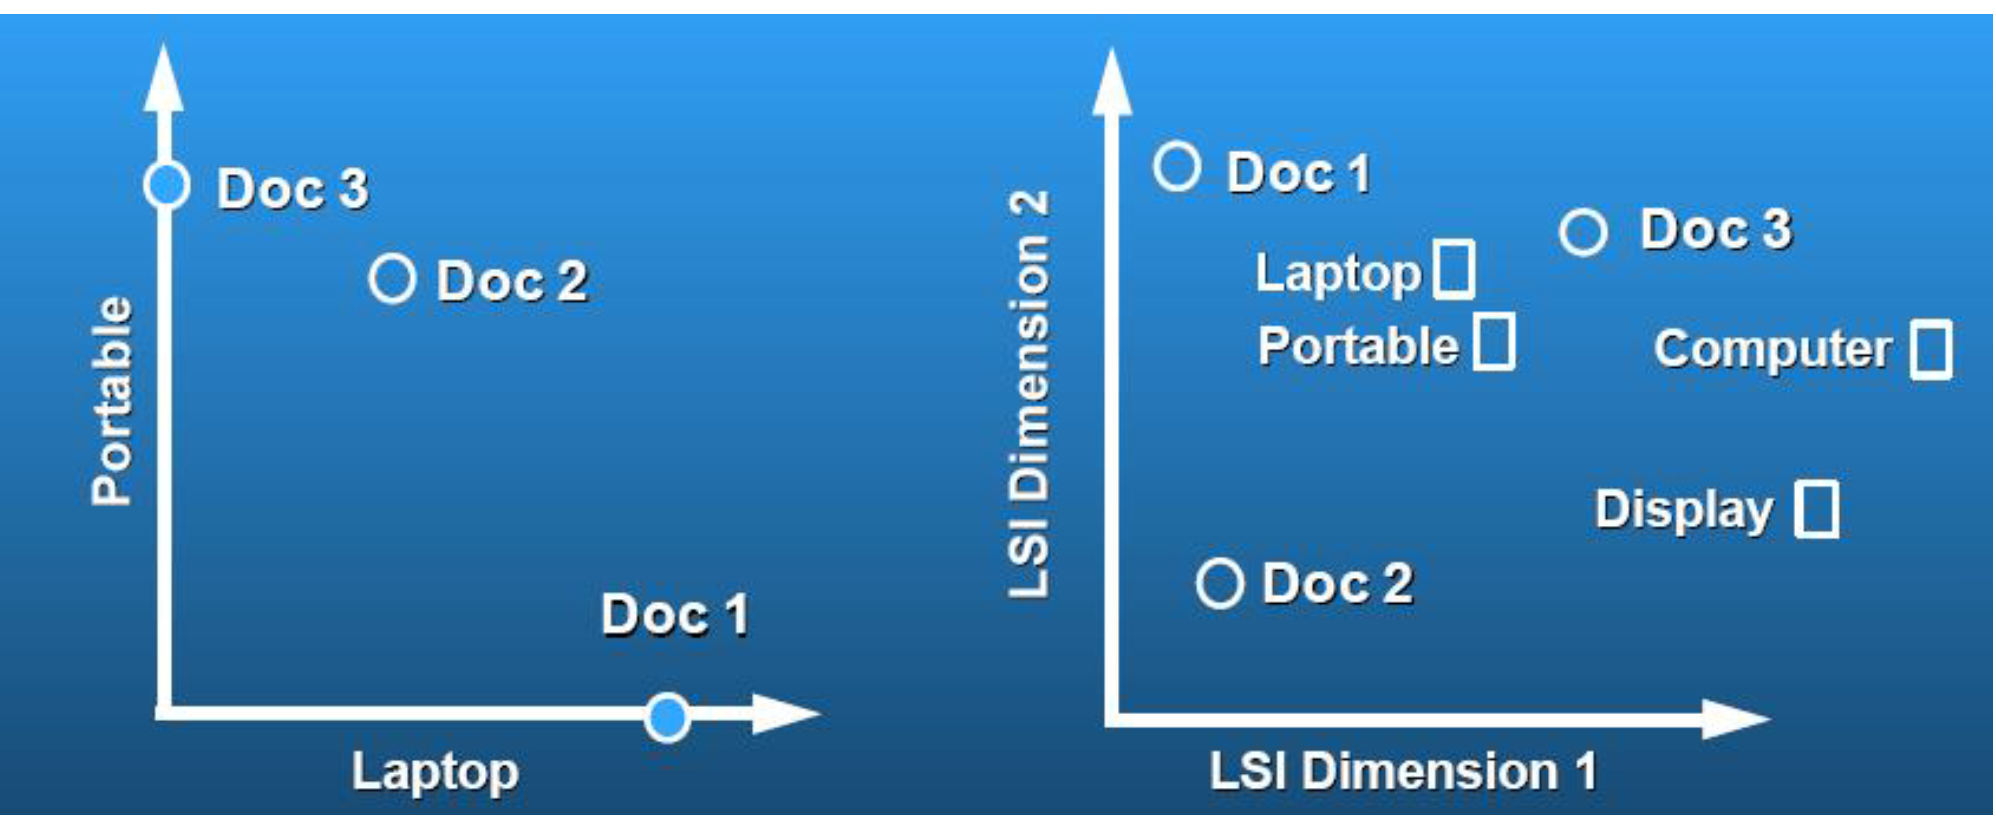
\includegraphics{img/lsa.png}
\caption{lsa}
\end{figure}

Grafik von Susan Dumais
(\href{http://www.ifis.uni-luebeck.de/~moeller/tuhh-lectures/mmieir-sose-12/05-Latent-Semantic-Analysis.pdf}{Quelle}).

    Das Ziel der LSA ist es, die Konzepte innerhalb der Dokumente zu finden.
Dabei greift das Verfahren auf eine Technik der linearen Algebra zurück,
der \textbf{Singulärwertzerlegung} (englisch: Singular Value
Decomposition). Die Idee dabei ist, dass die Term-Dokument Matrix aus
\textbf{Hauptdimensionen}, welche die wichtigen Konzepte der Dokumente
beinhalten, und aus weniger aussagekräftigen Dimensionen mit unwichtigen
Termen besteht. Mithilfe der Singulärwertzerlegung wird die originale
Term-Dokument Matrix in drei Matrizen aufgeteilt, wobei die beiden
äußeren Matrizen aus den linken bzw. rechten orthonormalen Eigenvektoren
bestehen und die mittlere Matrix eine Diagonalmatrix ist, die die
singulären Werte der Originalmatrix enthält. Mit Hilfe dieser Zerlegung
kann eine \textbf{Approximation} der Originalmatrix mit einer kleiner
dimensionierten Matrix erreicht werden. Die singulären Werte in der
Diagonalmatrix sind nach ihrer Größe absteigend geordnet. Singulärwerte,
die unter einem bestimmten Schwellenwert liegen, werden entfernt. Auch
in den anderen Matrizen werden entsprechende Zeilen oder Spalten
entfernt. Mit Hilfe der reduzierten Matrizen erhält man durch
Matrixmultiplikation die optimale Approximation der Originalmatrix, die
kleiner als die originale Term-Dokument Matrix ist, da Informationen aus
den weniger aussagekräftigen Dimensionen verworfen wurden. Weiterhin
werden bei der Dimensionsreduktion auch ähnliche Konzepte
zusammengefasst, so werden z.B. Worte wie ``Tür'' und ``Tor'' in einem
Konzept zusammengefasst.

Der Vorteil der LSA ist, dass anders als beim Bag-of-Words Modell die
\textbf{Semantik} der Dokumente wiedergegeben werden kann. Zudem werden
\textbf{Synonyme} zusammengefasst. Probleme hat LSA jedoch mit der
\textbf{Polysemie}. Zudem ist der Algorithmus sehr rechenaufwendig.

    \hypertarget{word-embeddings}{%
\section{Word Embeddings}\label{word-embeddings}}

\hypertarget{allgemeines}{%
\subsection{Allgemeines}\label{allgemeines}}

\textbf{Word Embeddings} (deutsch: Worteinbettungen) sind die
Sammelbezeichnung für eine Reihe von Sprachmodellierungstechniken.
Anders als beim Bag-of-Words Modell werden Wörter mit ähnlichen
Bedeutungen ähnlich dargestellt, wobei der Kontext der Wörter
berücksichtigt wird. Word Embeddings repräsentieren Wörter als Vektoren
in einem multidimensionalen semantischen Raum. In diesem Raum werden
Wörter, die ähnlich zueinander sind, näher beieinander platziert. Die
grundsätzliche Idee von Word Embeddings basiert auf der
\textbf{Distributionellen Hypothese} von John Rupert Firth, die besagt,
dass die Bedeutung eines Wortes durch sein Umfeld geprägt ist. Wörter,
die einen ähnlichen Kontext besitzen, haben eine ähnliche Bedeutung.
Anders als vorherige Vektorisierungsmethoden basieren Word Embeddings
auf \textbf{Vorhersagemodellen} (englisch: \textbf{prediction
models})Section \ref{fn2}, indem Wörter durch Wahrscheinlichkeiten
anstatt durch Häufigkeiten wie beim Bag-of-Words Modell oder bei der
Latent Semantic Analysis dargestellt werden. Weiterhin sind die
Wortvektoren von Word Embeddings anders als beim Bag-of-Words Modell
\textbf{dichtbesetzt} (englisch: \textbf{dense}) und haben weitaus
weniger Dimensionen (100-800 Dimensionen anstatt 100000-1000000, je nach
der Größe des Vokabulars). Dadurch haben die Wortvektoren eine viel
geringere Größe, bieten trotzdem eine effizientere und komplexere
Darstellung der Wörter.

Eine weitere Besonderheit von Word Embeddings ist, dass es mit diesen
möglich ist, eine Arithmetik mit Wörtern umzusetzen. So kann mit
Wortvektoren ``gerechnet'' werden. Folgende Gleichungen sind mit Word
Embeddings möglich:

\texttt{König\ -\ Mann\ +\ Frau\ =\ Königin}

\texttt{London\ -\ Großbritannien\ +\ Deutschland\ =\ Berlin}

Word Embeddings wurden ab 2013 durch die Einführung des Algorithmus
\textbf{Word2Vec} populär, in den Jahren darauf folgten weitere Word
Embedding Algorithmen wie \textbf{GloVe}, \textbf{FastText},
\textbf{ELMo} und \textbf{BERT}. In der folgenden Tabelle sind die
wichtigsten Unterschiede der hier erläuterten Embeddings
zusammengefasst, genauere Erläuterungen dieser Embeddings finden sich in
den folgenden Kapiteln. Die darauffolgende Abbildung liefert eine Art
Stammbaum der verschiedenen Embedding-Arten.

\hypertarget{fn2}{}
2 ~Obwohl GloVe eigentlich kein Vorhersagemodell verwendet,
unterscheidet sich GloVe trotzdem stark von vorhergehenden,
Häufigkeits-basierenden Modellen, weshalb es oft als Vohersagemodell
angesehen wird, siehe LEVY et. al.~(2015), Improving Distributional
Similarity with Lessons Learned from Word Embeddings,
https://levyomer.files.wordpress.com/2015/03/improving-distributional-similarity-tacl-2015.pdf
(abgerufen am 31.07.2020).

    TODO: ausfüllen \& mehr, gucken wie anders dargestellt werden kann

Word2Vec

GloVe

FastText

ELMo

BERT

Entstehungsjahr

2013

2014

2016

2018

2018

Out of vocabulary Fehler

ja

ja

nein

nein

nein

Kontextsensitiv

nein

nein

nein

ja

ja

gelernte Repräsentationen

Wörter

Wörter

Teilwörter

Wörter

Teilwörter

    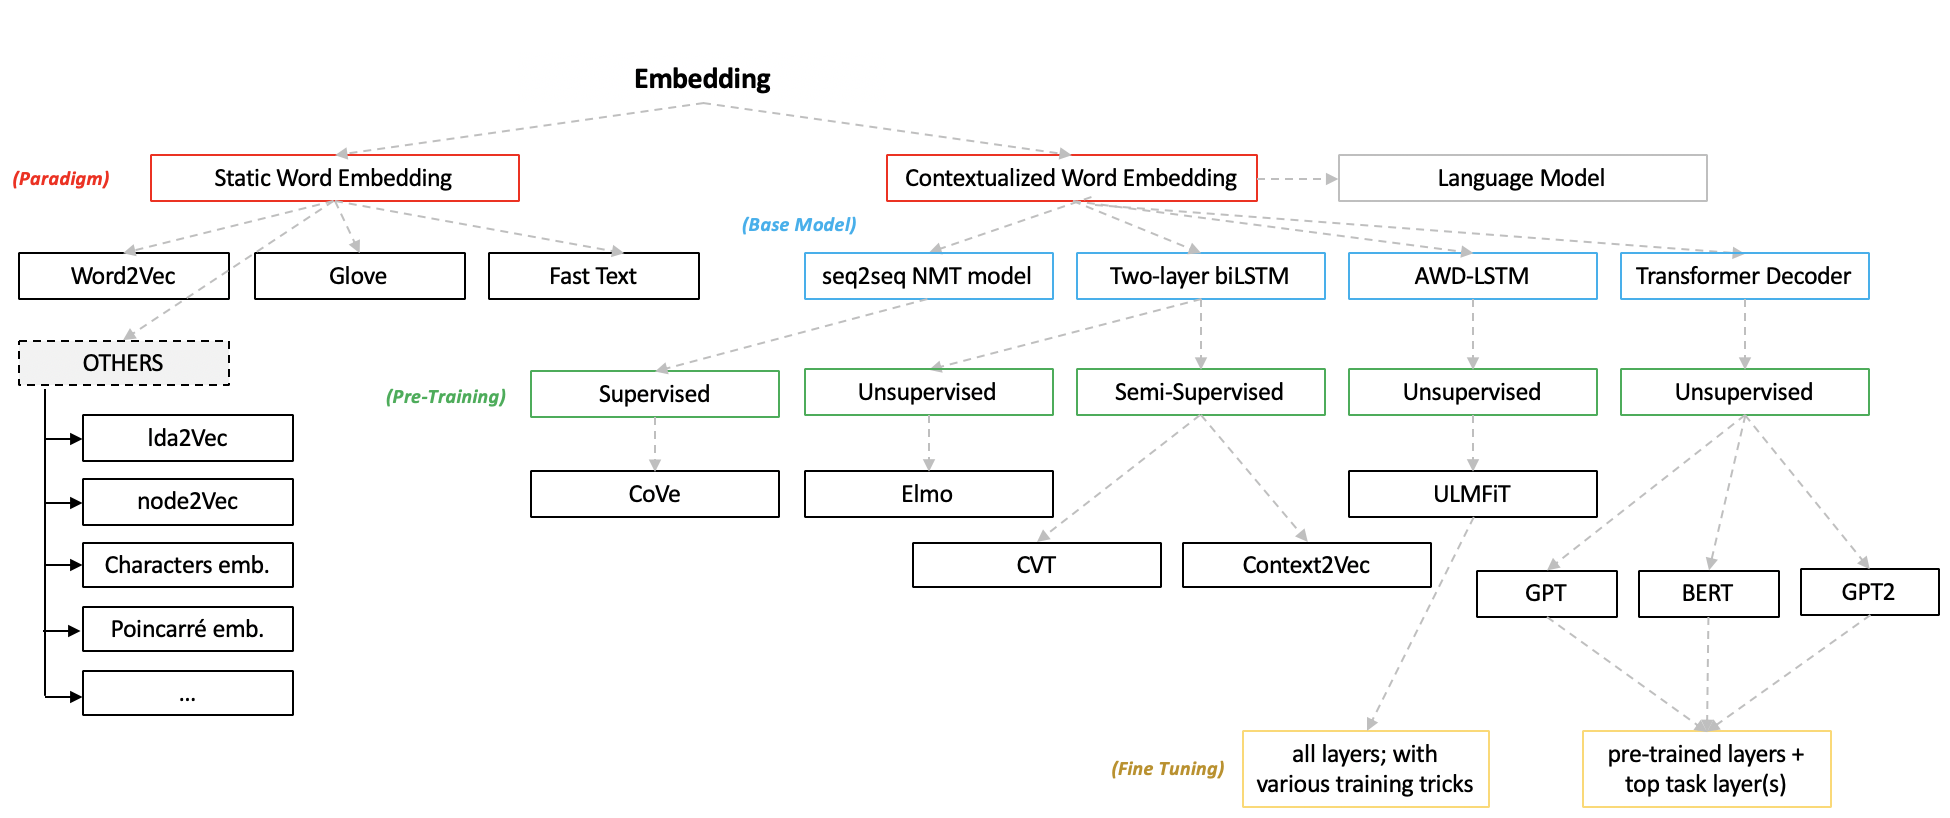
\includegraphics{img/all_embeddings.png}

Die Grafik wurde von dieser
\href{https://towardsdatascience.com/from-pre-trained-word-embeddings-to-pre-trained-language-models-focus-on-bert-343815627598}{Webseite}
entnommen.

    \hypertarget{word2vec}{%
\subsection{Word2Vec}\label{word2vec}}

Die Popularität von Word Embeddings ist vor allem \textbf{Word2Vec}
geschuldet, welches 2013 von Tomas Mikolov und weiteren Mitgliedern von
Google publiziert wurde (\href{https://arxiv.org/abs/1301.3781}{Paper}).
Word2Vec basiert auf einer simplen und effektiven Feedforward Neuronalen
Netzstruktur. Word2Vec implementiert zwei verschiedene Ansätze zur
Berechnung der Wortwahrscheinlichkeiten: \textbf{Continous Bag of Words}
(\textbf{CBOW}) und das \textbf{Skip-gram Modell}.

\textbf{Continous Bag of Words} versucht die Wahrscheinlichkeit eines
Wortes oder einer Gruppe von Wörtern anhand eines gegebenen Kontext
vorauszusagen:

\begin{figure}
\centering
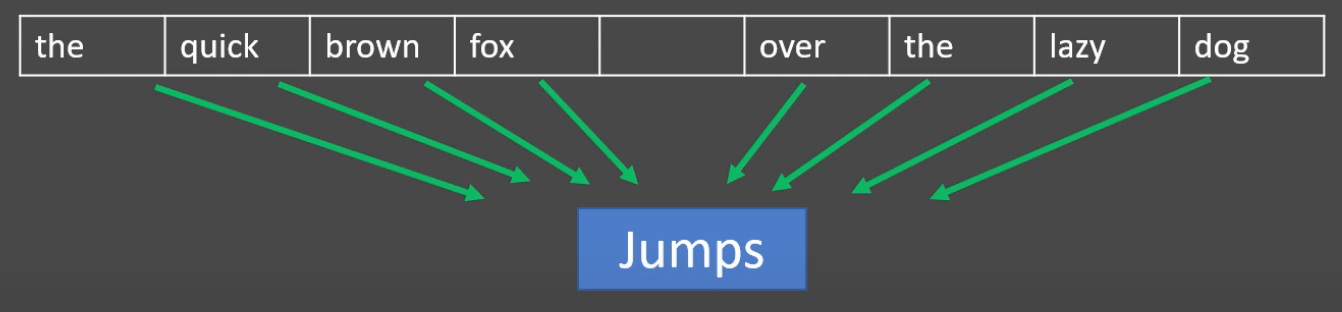
\includegraphics{img/cbow.png}
\caption{cbow}
\end{figure}

Das \textbf{Skip-gram Model} funktioniert wie CBOW, nur anders herum.
Das Modell versucht, anhand eines gegebenen Wortes den Kontext
vorauszusagen:

\begin{figure}
\centering
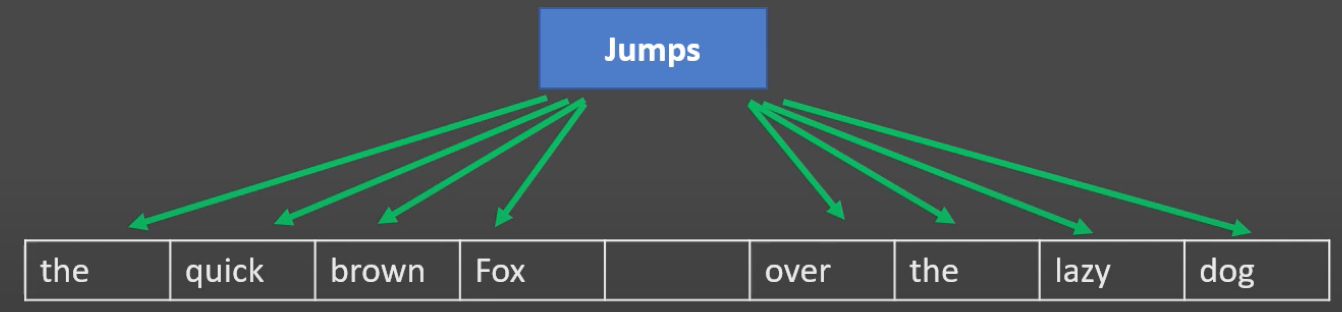
\includegraphics{img/skipgram.png}
\caption{skip-gram}
\end{figure}

Word2Vec nutzt wahlweise eine dieser Techniken, um aus rohen Textdaten
mithilfe eines Neuronalen Netzes Wortvektoren zu erstellen. Dabei kann
Word2Vec bei vielen Implementierungen (z.b. bei Gensim) auf zwei Arten
verwendet werden: Entweder werden bereits vortrainierte Embeddings
geladen oder es werden eigene Embeddings auf eigenen Textdaten
trainiert.

    \hypertarget{vortrainierte-embeddings-verwenden}{%
\subsubsection{Vortrainierte Embeddings
verwenden}\label{vortrainierte-embeddings-verwenden}}

Für die Demonstration der Nutzung von vortrainierten Word Embeddings
wird ein deutsches Modell verwendet, welches auf Wikipedia- und
Zeitungsartikeln trainiert wurde
(\href{https://devmount.github.io/GermanWordEmbeddings/}{Quelle}). Als
Framework wird \textbf{Gensim} verwendet.

    \begin{tcolorbox}[breakable, size=fbox, boxrule=1pt, pad at break*=1mm,colback=cellbackground, colframe=cellborder]
\prompt{In}{incolor}{54}{\boxspacing}
\begin{Verbatim}[commandchars=\\\{\}]
\PY{n}{pre\PYZus{}w2v} \PY{o}{=} \PY{n}{gensim}\PY{o}{.}\PY{n}{models}\PY{o}{.}\PY{n}{KeyedVectors}\PY{o}{.}\PY{n}{load\PYZus{}word2vec\PYZus{}format}\PY{p}{(}\PY{l+s+s1}{\PYZsq{}}\PY{l+s+s1}{german\PYZus{}model.bin}\PY{l+s+s1}{\PYZsq{}}\PY{p}{,} 
                                                          \PY{n}{binary}\PY{o}{=}\PY{k+kc}{True}\PY{p}{)}
\end{Verbatim}
\end{tcolorbox}

    Im folgenden Code werden die 5 ähnlichsten Wörter zu ``König''
ausgegeben. Alle diese Wörter passen auch thematisch zu ``König'', sie
verbindet alle das Thema ``royal'' bzw. ``Königshaus''.

    \begin{tcolorbox}[breakable, size=fbox, boxrule=1pt, pad at break*=1mm,colback=cellbackground, colframe=cellborder]
\prompt{In}{incolor}{55}{\boxspacing}
\begin{Verbatim}[commandchars=\\\{\}]
\PY{k}{for} \PY{n}{t} \PY{o+ow}{in} \PY{n}{pre\PYZus{}w2v}\PY{o}{.}\PY{n}{most\PYZus{}similar}\PY{p}{(}\PY{l+s+s1}{\PYZsq{}}\PY{l+s+s1}{Koenig}\PY{l+s+s1}{\PYZsq{}}\PY{p}{,} \PY{n}{topn}\PY{o}{=}\PY{l+m+mi}{5}\PY{p}{)}\PY{p}{:} 
    \PY{n+nb}{print}\PY{p}{(}\PY{l+s+sa}{f}\PY{l+s+s2}{\PYZdq{}}\PY{l+s+si}{\PYZob{}}\PY{n}{t}\PY{p}{[}\PY{l+m+mi}{0}\PY{p}{]}\PY{l+s+si}{\PYZcb{}}\PY{l+s+s2}{: }\PY{l+s+si}{\PYZob{}}\PY{n}{np}\PY{o}{.}\PY{n}{around}\PY{p}{(}\PY{n}{t}\PY{p}{[}\PY{l+m+mi}{1}\PY{p}{]}\PY{p}{,} \PY{n}{decimals}\PY{o}{=}\PY{l+m+mi}{3}\PY{p}{)}\PY{l+s+si}{\PYZcb{}}\PY{l+s+s2}{\PYZdq{}}\PY{p}{)}
\end{Verbatim}
\end{tcolorbox}

    \begin{Verbatim}[commandchars=\\\{\}]
Prinz: 0.786
Koenigs: 0.736
Koenigin: 0.726
Jungkoenig: 0.705
Kaiser: 0.705
    \end{Verbatim}

    Auch das Rechenbeispiel aus Kapitel 3.1 kann mit Word2Vec umgesetzt
werden. Addiert man ``König'' mit ``Frau'' und subtrahiert ``Mann'',
erhält man Begriffe zum Thema ``Königin''.

    \begin{tcolorbox}[breakable, size=fbox, boxrule=1pt, pad at break*=1mm,colback=cellbackground, colframe=cellborder]
\prompt{In}{incolor}{56}{\boxspacing}
\begin{Verbatim}[commandchars=\\\{\}]
\PY{k}{for} \PY{n}{t} \PY{o+ow}{in} \PY{n}{pre\PYZus{}w2v}\PY{o}{.}\PY{n}{most\PYZus{}similar}\PY{p}{(}\PY{n}{positive}\PY{o}{=}\PY{p}{[}\PY{l+s+s1}{\PYZsq{}}\PY{l+s+s1}{Koenig}\PY{l+s+s1}{\PYZsq{}}\PY{p}{,} \PY{l+s+s1}{\PYZsq{}}\PY{l+s+s1}{Frau}\PY{l+s+s1}{\PYZsq{}}\PY{p}{]}\PY{p}{,}
                              \PY{n}{negative}\PY{o}{=}\PY{p}{[}\PY{l+s+s1}{\PYZsq{}}\PY{l+s+s1}{Mann}\PY{l+s+s1}{\PYZsq{}}\PY{p}{]}\PY{p}{,} \PY{n}{topn}\PY{o}{=}\PY{l+m+mi}{5}\PY{p}{)}\PY{p}{:}
    \PY{n+nb}{print}\PY{p}{(}\PY{l+s+sa}{f}\PY{l+s+s2}{\PYZdq{}}\PY{l+s+si}{\PYZob{}}\PY{n}{t}\PY{p}{[}\PY{l+m+mi}{0}\PY{p}{]}\PY{l+s+si}{\PYZcb{}}\PY{l+s+s2}{: }\PY{l+s+si}{\PYZob{}}\PY{n}{np}\PY{o}{.}\PY{n}{around}\PY{p}{(}\PY{n}{t}\PY{p}{[}\PY{l+m+mi}{1}\PY{p}{]}\PY{p}{,} \PY{n}{decimals}\PY{o}{=}\PY{l+m+mi}{3}\PY{p}{)}\PY{l+s+si}{\PYZcb{}}\PY{l+s+s2}{\PYZdq{}}\PY{p}{)}
\end{Verbatim}
\end{tcolorbox}

    \begin{Verbatim}[commandchars=\\\{\}]
Koenigin: 0.752
Prinzessin: 0.715
Prinz: 0.688
Jungschuetzenkoenigin: 0.674
Majestaet: 0.659
    \end{Verbatim}

    Weiterhin kann man auch ein Wort mit einer Liste von anderen Wörtern
vergleichen und abfragen, welchem Wort aus der Liste das Wort am
ähnlichsten ist oder aber man überprüft bei einer Liste von Wörtern,
welches Wort nicht passt.

    \begin{tcolorbox}[breakable, size=fbox, boxrule=1pt, pad at break*=1mm,colback=cellbackground, colframe=cellborder]
\prompt{In}{incolor}{59}{\boxspacing}
\begin{Verbatim}[commandchars=\\\{\}]
\PY{n}{most\PYZus{}similar} \PY{o}{=} \PY{n}{pre\PYZus{}w2v}\PY{o}{.}\PY{n}{most\PYZus{}similar\PYZus{}to\PYZus{}given}\PY{p}{(}\PY{l+s+s1}{\PYZsq{}}\PY{l+s+s1}{Banane}\PY{l+s+s1}{\PYZsq{}}\PY{p}{,} \PY{p}{[}\PY{l+s+s1}{\PYZsq{}}\PY{l+s+s1}{Koenig}\PY{l+s+s1}{\PYZsq{}}\PY{p}{,} \PY{l+s+s1}{\PYZsq{}}\PY{l+s+s1}{Berg}\PY{l+s+s1}{\PYZsq{}}\PY{p}{,} 
                                                        \PY{l+s+s1}{\PYZsq{}}\PY{l+s+s1}{Haus}\PY{l+s+s1}{\PYZsq{}}\PY{p}{,} \PY{l+s+s1}{\PYZsq{}}\PY{l+s+s1}{Apfel}\PY{l+s+s1}{\PYZsq{}}\PY{p}{]}\PY{p}{)}
\PY{n}{doesnt\PYZus{}match} \PY{o}{=} \PY{n}{pre\PYZus{}w2v}\PY{o}{.}\PY{n}{doesnt\PYZus{}match}\PY{p}{(}\PY{p}{[}\PY{l+s+s1}{\PYZsq{}}\PY{l+s+s1}{Koenig}\PY{l+s+s1}{\PYZsq{}}\PY{p}{,} \PY{l+s+s1}{\PYZsq{}}\PY{l+s+s1}{Thron}\PY{l+s+s1}{\PYZsq{}}\PY{p}{,} \PY{l+s+s1}{\PYZsq{}}\PY{l+s+s1}{Berg}\PY{l+s+s1}{\PYZsq{}}\PY{p}{,} \PY{l+s+s1}{\PYZsq{}}\PY{l+s+s1}{Prinzessin}\PY{l+s+s1}{\PYZsq{}}\PY{p}{]}\PY{p}{)}
\PY{n+nb}{print}\PY{p}{(}\PY{l+s+sa}{f}\PY{l+s+s2}{\PYZdq{}}\PY{l+s+s2}{Welches Wort ist am ähnlichsten zu }\PY{l+s+s2}{\PYZsq{}}\PY{l+s+s2}{Banane}\PY{l+s+s2}{\PYZsq{}}\PY{l+s+s2}{? \PYZhy{}\PYZgt{} }\PY{l+s+si}{\PYZob{}}\PY{n}{most\PYZus{}similar}\PY{l+s+si}{\PYZcb{}}\PY{l+s+s2}{\PYZdq{}}\PY{p}{)}
\PY{n+nb}{print}\PY{p}{(}\PY{l+s+sa}{f}\PY{l+s+s2}{\PYZdq{}}\PY{l+s+s2}{Welches Wort passt nicht zu den anderen Wörtern? \PYZhy{}\PYZgt{} }\PY{l+s+si}{\PYZob{}}\PY{n}{doesnt\PYZus{}match}\PY{l+s+si}{\PYZcb{}}\PY{l+s+s2}{\PYZdq{}}\PY{p}{)}
\end{Verbatim}
\end{tcolorbox}

    \begin{Verbatim}[commandchars=\\\{\}]
Welches Wort ist am ähnlichsten zu 'Banane'? -> Apfel
Welches Wort passt nicht zu den anderen Wörtern? -> Berg
    \end{Verbatim}

    Plottet man die Wortvektoren der verwandten Wörter (hier die 5
ähnlichsten Wörter), werden die einzelnen Themen sehr gut sichtbar, da
sie Cluster bilden und von anderen Themen abgrenzen.

    \begin{tcolorbox}[breakable, size=fbox, boxrule=1pt, pad at break*=1mm,colback=cellbackground, colframe=cellborder]
\prompt{In}{incolor}{58}{\boxspacing}
\begin{Verbatim}[commandchars=\\\{\}]
\PY{n}{wordlist} \PY{o}{=} \PY{p}{[}\PY{l+s+s1}{\PYZsq{}}\PY{l+s+s1}{Haus}\PY{l+s+s1}{\PYZsq{}}\PY{p}{,} \PY{l+s+s1}{\PYZsq{}}\PY{l+s+s1}{Berg}\PY{l+s+s1}{\PYZsq{}}\PY{p}{,} \PY{l+s+s1}{\PYZsq{}}\PY{l+s+s1}{Koenig}\PY{l+s+s1}{\PYZsq{}}\PY{p}{,} \PY{l+s+s1}{\PYZsq{}}\PY{l+s+s1}{gehen}\PY{l+s+s1}{\PYZsq{}}\PY{p}{]}
\PY{n}{plot\PYZus{}word\PYZus{}embeddings}\PY{p}{(}\PY{n}{pre\PYZus{}w2v}\PY{p}{,} \PY{n}{wordlist}\PY{p}{,} \PY{n}{figsize}\PY{o}{=}\PY{p}{(}\PY{l+m+mi}{8}\PY{p}{,}\PY{l+m+mi}{4}\PY{p}{)}\PY{p}{)}
\end{Verbatim}
\end{tcolorbox}

    \begin{center}
    \adjustimage{max size={0.9\linewidth}{0.9\paperheight}}{output_22_0.png}
    \end{center}
    { \hspace*{\fill} \\}
    
    \hypertarget{eigene-embeddings-trainieren}{%
\subsubsection{Eigene Embeddings
trainieren}\label{eigene-embeddings-trainieren}}

Es ist auch möglich, eigene Embeddings zu trainieren. Dabei muss sich
zuvor für die Technik \textbf{CBOW} oder \textbf{Skip-gram} entschieden
werden (wird durch den Parameter \texttt{sg}gesteuert). Es wurde der
englische Datensatz \textbf{Amazon Reviews} verwendet
(\href{https://nijianmo.github.io/amazon/index.html}{Quelle}). Dieser
wurde für Demonstrationszwecke auf Reviews zu elektronischen Geräten aus
dem Jahr 2018 gekürzt. Auch hier passen die ähnlichsten 5 Wörter sehr
gut zum ausgewählten Wort \emph{smartphone}.

    \begin{tcolorbox}[breakable, size=fbox, boxrule=1pt, pad at break*=1mm,colback=cellbackground, colframe=cellborder]
\prompt{In}{incolor}{10}{\boxspacing}
\begin{Verbatim}[commandchars=\\\{\}]
\PY{o}{\PYZpc{}\PYZpc{}time}
\PY{n}{word2vec\PYZus{}cbow} \PY{o}{=} \PY{n}{Word2Vec}\PY{p}{(}\PY{n}{texts}\PY{p}{,} \PY{n}{min\PYZus{}count}\PY{o}{=}\PY{l+m+mi}{1}\PY{p}{,} \PY{n}{size}\PY{o}{=}\PY{l+m+mi}{100}\PY{p}{,} \PY{n}{window}\PY{o}{=}\PY{l+m+mi}{5}\PY{p}{,} \PY{n}{sg}\PY{o}{=}\PY{l+m+mi}{0}\PY{p}{)}
\PY{n}{word2vec\PYZus{}skipgram} \PY{o}{=} \PY{n}{Word2Vec}\PY{p}{(}\PY{n}{texts}\PY{p}{,} \PY{n}{min\PYZus{}count}\PY{o}{=}\PY{l+m+mi}{1}\PY{p}{,} \PY{n}{size}\PY{o}{=}\PY{l+m+mi}{100}\PY{p}{,} \PY{n}{window}\PY{o}{=}\PY{l+m+mi}{5}\PY{p}{,} \PY{n}{sg}\PY{o}{=}\PY{l+m+mi}{1}\PY{p}{)}
\end{Verbatim}
\end{tcolorbox}

    \begin{Verbatim}[commandchars=\\\{\}]
CPU times: user 6min 16s, sys: 5.09 s, total: 6min 21s
Wall time: 3min 30s
    \end{Verbatim}

    \begin{tcolorbox}[breakable, size=fbox, boxrule=1pt, pad at break*=1mm,colback=cellbackground, colframe=cellborder]
\prompt{In}{incolor}{11}{\boxspacing}
\begin{Verbatim}[commandchars=\\\{\}]
\PY{n}{word2vec\PYZus{}cbow}\PY{o}{.}\PY{n}{wv}\PY{o}{.}\PY{n}{most\PYZus{}similar}\PY{p}{(}\PY{l+s+s1}{\PYZsq{}}\PY{l+s+s1}{phone}\PY{l+s+s1}{\PYZsq{}}\PY{p}{,} \PY{n}{topn}\PY{o}{=}\PY{l+m+mi}{5}\PY{p}{)}
\end{Verbatim}
\end{tcolorbox}

            \begin{tcolorbox}[breakable, size=fbox, boxrule=.5pt, pad at break*=1mm, opacityfill=0]
\prompt{Out}{outcolor}{11}{\boxspacing}
\begin{Verbatim}[commandchars=\\\{\}]
[('iphone', 0.7328867316246033),
 ('cell', 0.6630538702011108),
 ('phones', 0.6511064767837524),
 ('smartphone', 0.6296558976173401),
 ('computer', 0.6081698536872864)]
\end{Verbatim}
\end{tcolorbox}
        
    \hypertarget{glove}{%
\subsection{GloVe}\label{glove}}

\textbf{GloVe} (= Global Vectors) wurde 2014 von Pennigton et.
al.~veröffentlicht
(\href{https://nlp.stanford.edu/pubs/glove.pdf}{Paper}). Vor der
Veröffentlichung von GloVe ließen sich die Wortvektorisierungsmethoden
in zwei Hauptströmungen unterteilen: das Statistik-basierende
\textbf{LDA}Section \ref{fn3} und das lernbasierte \textbf{Word2Vec}.
Während LDA Wörter mithilfe von Häufigkeiten in einer Kookkurrenz-Matrix
darstellt, verwendet Word2Vec zur Darstellung der Wörter
Wortwahrscheinlichkeiten, die mithilfe eines Voraussage-Modells erstellt
wurden. \textbf{GloVe} verwendet für die Darstellung der Häufigkeiten
wie LDA eine Kookkurrenz-Matrix, wobei GloVe die Häufigkeiten vorher
normalisiert und mithilfe des Logarithmus ``\emph{glättet}'' (englisch:
\emph{smoothing}). Anders als Word2Vec benutzt es für die Erstellung der
Embeddings also keine neuronalen Netze, die erst durch ein Training die
Wortbeziehungen erlernen, sondern die Beziehungen werden \textbf{global}
(daher auch der Name) mithilfe einer Mischung aus maschinellem Lernen
und statischen Verfahren aus den Texten gewonnen.

\hypertarget{fn3}{}
3 ~LDA steht für ``Latent Dirichlet allocation'' und ist ein
Algorithmus, der Wörter ähnlichen Gruppen anhand der Wahrscheinlichkeit,
dass sie zusammen in einem Dokument vorkommen, zuordnet.

    Für die Demonstatration der Glove-Embeddings wurde die Bibliothek
\textbf{Flair} verwendet. Jeder Vektor für jedes Token-Embedding hat
eine Länge von 100, es wurden jedoch nur die ersten drei Zahlen
ausgegeben.

    \begin{tcolorbox}[breakable, size=fbox, boxrule=1pt, pad at break*=1mm,colback=cellbackground, colframe=cellborder]
\prompt{In}{incolor}{22}{\boxspacing}
\begin{Verbatim}[commandchars=\\\{\}]
\PY{n}{string} \PY{o}{=} \PY{l+s+s2}{\PYZdq{}}\PY{l+s+s2}{smartphones have a touchscreen}\PY{l+s+s2}{\PYZdq{}}
\PY{n}{sentence} \PY{o}{=} \PY{n}{Sentence}\PY{p}{(}\PY{n}{string}\PY{p}{,} \PY{n}{use\PYZus{}tokenizer}\PY{o}{=}\PY{k+kc}{True}\PY{p}{)}
\PY{n}{glove\PYZus{}embeddings} \PY{o}{=} \PY{n}{WordEmbeddings}\PY{p}{(}\PY{l+s+s1}{\PYZsq{}}\PY{l+s+s1}{glove}\PY{l+s+s1}{\PYZsq{}}\PY{p}{)}\PY{o}{.}\PY{n}{embed}\PY{p}{(}\PY{n}{sentence}\PY{p}{)}

\PY{k}{for} \PY{n}{token} \PY{o+ow}{in} \PY{n}{sentence}\PY{p}{:}
    \PY{n+nb}{print}\PY{p}{(}\PY{l+s+sa}{f}\PY{l+s+s2}{\PYZdq{}}\PY{l+s+s2}{\PYZsq{}}\PY{l+s+si}{\PYZob{}}\PY{n}{token}\PY{o}{.}\PY{n}{text}\PY{l+s+si}{\PYZcb{}}\PY{l+s+s2}{\PYZsq{}}\PY{l+s+s2}{: }\PY{l+s+si}{\PYZob{}}\PY{n}{token}\PY{o}{.}\PY{n}{embedding}\PY{p}{[}\PY{p}{:}\PY{l+m+mi}{3}\PY{p}{]}\PY{l+s+si}{\PYZcb{}}\PY{l+s+s2}{ }\PY{l+s+s2}{\PYZdq{}} \PY{o}{+}
          \PY{l+s+sa}{f}\PY{l+s+s2}{\PYZdq{}}\PY{l+s+s2}{(Vektorlänge: }\PY{l+s+si}{\PYZob{}}\PY{n+nb}{len}\PY{p}{(}\PY{n}{token}\PY{o}{.}\PY{n}{embedding}\PY{p}{)}\PY{l+s+si}{\PYZcb{}}\PY{l+s+s2}{)}\PY{l+s+s2}{\PYZdq{}}\PY{p}{)}
\end{Verbatim}
\end{tcolorbox}

    \begin{Verbatim}[commandchars=\\\{\}]
'smartphones': tensor([-0.2138, -0.3245,  0.2806]) (Vektorlänge: 100)
'have': tensor([0.1571, 0.6561, 0.0021]) (Vektorlänge: 100)
'a': tensor([-0.2709,  0.0440, -0.0203]) (Vektorlänge: 100)
'touchscreen': tensor([-0.7974,  0.1240,  0.7148]) (Vektorlänge: 100)
    \end{Verbatim}

    \hypertarget{fasttext}{%
\subsection{FastText}\label{fasttext}}

\textbf{Word2Vec} und \textbf{GloVe} haben Probleme damit, unbekannte
Wörter zu verarbeiten. Dieser Fehler nennt sich \textbf{out of
vocabulary} (\textbf{OOV}), da das Wort nicht im bekannten Vokabular der
Embeddings vorkommt. Es ist zwar möglich, unbekannten Wörtern ein
zufälliges Embedding zuzuweisen, jedoch ist dies vor allem
problematisch, wenn das unbekannte Wort ein Schlüsselwort im
untersuchten Text ist. Eine Embedding Verfahren, welches das OOV Problem
löst, ist \textbf{FastText}, welches 2016 von Bojanowski et.
al.~veröffentlicht wurde
(\href{https://arxiv.org/abs/1607.04606}{Paper}). FastText löst das
OOV-Problem, indem es Wörter mithilfe von Buchstaben N-Grammen in
einzelne Teilwörter aufteilt. Während des Trainings lernt FastText die
Buchstaben N-Gramme der Teilwörter. Bei einem unbekannten Wort wird ein
Embedding dieses Wortes erzeugt, indem der Mittelwert der
Vektorrepräsentationen der verschiedenen Buchstaben N-Gramm-Embeddings
gebildet wird. Zwar kann FastText so mit unbekannten Wörtern umgehen,
eine optimale Lösung für das Problem ist dies jedoch nicht, da Wörter
zwar aus ähnlichen Buchstaben N-Gramm-Bestandteilen bestehen, sich aber
semantisch trotzdem stark voneinander unterscheiden können.

Im Folgenden wird die Funktionsweise von FastText-Embeddings anhand
eines Beispielsatzes demonstriert. Wie bei den GloVe-Embeddings auch
wird hier die Bibliothek \textbf{Flair} verwendet. Der folgende Code
erzeugt sowohl für das FastText-Embedding als auch für das
GloVe-Embedding einen OOV-Fehler für das Wort ``tensorflow'',
dargestellt durch einen Wortvektor, der nur aus Nullen besteht.

    \begin{tcolorbox}[breakable, size=fbox, boxrule=1pt, pad at break*=1mm,colback=cellbackground, colframe=cellborder]
\prompt{In}{incolor}{44}{\boxspacing}
\begin{Verbatim}[commandchars=\\\{\}]
\PY{n}{string2} \PY{o}{=} \PY{l+s+s2}{\PYZdq{}}\PY{l+s+s2}{tensorflow is a library}\PY{l+s+s2}{\PYZdq{}}
\PY{n}{sentence2} \PY{o}{=} \PY{n}{Sentence}\PY{p}{(}\PY{n}{string2}\PY{p}{,} \PY{n}{use\PYZus{}tokenizer}\PY{o}{=}\PY{k+kc}{True}\PY{p}{)}
\PY{n}{sentence3} \PY{o}{=} \PY{n}{Sentence}\PY{p}{(}\PY{n}{string2}\PY{p}{,} \PY{n}{use\PYZus{}tokenizer}\PY{o}{=}\PY{k+kc}{True}\PY{p}{)}
\PY{n}{glove\PYZus{}embedding2} \PY{o}{=} \PY{n}{WordEmbeddings}\PY{p}{(}\PY{l+s+s1}{\PYZsq{}}\PY{l+s+s1}{glove}\PY{l+s+s1}{\PYZsq{}}\PY{p}{)}\PY{o}{.}\PY{n}{embed}\PY{p}{(}\PY{n}{sentence2}\PY{p}{)}
\PY{n}{fasttext\PYZus{}embedding2} \PY{o}{=} \PY{n}{WordEmbeddings}\PY{p}{(}\PY{l+s+s1}{\PYZsq{}}\PY{l+s+s1}{en}\PY{l+s+s1}{\PYZsq{}}\PY{p}{)}\PY{o}{.}\PY{n}{embed}\PY{p}{(}\PY{n}{sentence3}\PY{p}{)}

\PY{k}{for} \PY{n}{token1}\PY{p}{,} \PY{n}{token2} \PY{o+ow}{in} \PY{n+nb}{zip}\PY{p}{(}\PY{n}{sentence2}\PY{p}{,} \PY{n}{sentence3}\PY{p}{)}\PY{p}{:}
    \PY{n+nb}{print}\PY{p}{(}\PY{l+s+sa}{f}\PY{l+s+s2}{\PYZdq{}}\PY{l+s+s2}{[GloVe] }\PY{l+s+s2}{\PYZsq{}}\PY{l+s+si}{\PYZob{}}\PY{n}{token1}\PY{o}{.}\PY{n}{text}\PY{l+s+si}{\PYZcb{}}\PY{l+s+s2}{\PYZsq{}}\PY{l+s+s2}{: }\PY{l+s+si}{\PYZob{}}\PY{n}{token1}\PY{o}{.}\PY{n}{embedding}\PY{p}{[}\PY{p}{:}\PY{l+m+mi}{3}\PY{p}{]}\PY{l+s+si}{\PYZcb{}}\PY{l+s+s2}{ }\PY{l+s+s2}{\PYZdq{}} \PY{o}{+}
          \PY{l+s+sa}{f}\PY{l+s+s2}{\PYZdq{}}\PY{l+s+s2}{(Vektorlänge: }\PY{l+s+si}{\PYZob{}}\PY{n+nb}{len}\PY{p}{(}\PY{n}{token1}\PY{o}{.}\PY{n}{embedding}\PY{p}{)}\PY{l+s+si}{\PYZcb{}}\PY{l+s+s2}{)}\PY{l+s+s2}{\PYZdq{}}\PY{p}{)}
    \PY{n+nb}{print}\PY{p}{(}\PY{l+s+sa}{f}\PY{l+s+s2}{\PYZdq{}}\PY{l+s+s2}{[FastText] }\PY{l+s+s2}{\PYZsq{}}\PY{l+s+si}{\PYZob{}}\PY{n}{token2}\PY{o}{.}\PY{n}{text}\PY{l+s+si}{\PYZcb{}}\PY{l+s+s2}{\PYZsq{}}\PY{l+s+s2}{: }\PY{l+s+si}{\PYZob{}}\PY{n}{token2}\PY{o}{.}\PY{n}{embedding}\PY{p}{[}\PY{p}{:}\PY{l+m+mi}{3}\PY{p}{]}\PY{l+s+si}{\PYZcb{}}\PY{l+s+s2}{ }\PY{l+s+s2}{\PYZdq{}} \PY{o}{+}
          \PY{l+s+sa}{f}\PY{l+s+s2}{\PYZdq{}}\PY{l+s+s2}{(Vektorlänge: }\PY{l+s+si}{\PYZob{}}\PY{n+nb}{len}\PY{p}{(}\PY{n}{token2}\PY{o}{.}\PY{n}{embedding}\PY{p}{)}\PY{l+s+si}{\PYZcb{}}\PY{l+s+s2}{)}\PY{l+s+s2}{\PYZdq{}}\PY{p}{)}
    \PY{k}{break}
\end{Verbatim}
\end{tcolorbox}

    \begin{Verbatim}[commandchars=\\\{\}]
[GloVe] 'tensorflow': tensor([0., 0., 0.]) (Vektorlänge: 100)
[FastText] 'tensorflow': tensor([0., 0., 0.]) (Vektorlänge: 300)
    \end{Verbatim}

    Um keinen OOV-Fehler zu erzeugen, muss anstatt der Klasse
\texttt{WordEmbeddings} die Klasse \texttt{FastTextEmbeddings} in
Kombination mit einem selbst heruntergeladen englischen Model verwendet
werden (\href{https://fasttext.cc/docs/en/pretrained-vectors.html}{Link
zum Modell}). Nun kann das Wort ``tensorflow'' dargestellt
werden.Section \ref{fn4}

\hypertarget{fn4}{}
4 ~Da die FastText-Embeddings sehr groß sind, wurden die Wortvektoren
extern berechnet, hier werden nur die Ergebnisse angezeigt.

    \begin{tcolorbox}[breakable, size=fbox, boxrule=1pt, pad at break*=1mm,colback=cellbackground, colframe=cellborder]
\prompt{In}{incolor}{67}{\boxspacing}
\begin{Verbatim}[commandchars=\\\{\}]
\PY{c+c1}{\PYZsh{} sentence4 = Sentence(string2, use\PYZus{}tokenizer=True)}
\PY{c+c1}{\PYZsh{} fasttext\PYZus{}embedding = FastTextEmbeddings(\PYZsq{}cc.en.300.bin\PYZsq{}).embed(sentence4)}
\PY{k}{with} \PY{n+nb}{open}\PY{p}{(}\PY{l+s+s2}{\PYZdq{}}\PY{l+s+s2}{fasttext.json}\PY{l+s+s2}{\PYZdq{}}\PY{p}{,} \PY{l+s+s2}{\PYZdq{}}\PY{l+s+s2}{r}\PY{l+s+s2}{\PYZdq{}}\PY{p}{)} \PY{k}{as} \PY{n}{f}\PY{p}{:}
    \PY{n}{sentence4\PYZus{}worddict} \PY{o}{=} \PY{n}{json}\PY{o}{.}\PY{n}{load}\PY{p}{(}\PY{n}{f}\PY{p}{)}
    \PY{k}{for} \PY{n}{k}\PY{p}{,} \PY{n}{v} \PY{o+ow}{in} \PY{n}{sentence4\PYZus{}worddict}\PY{o}{.}\PY{n}{items}\PY{p}{(}\PY{p}{)}\PY{p}{:}
         \PY{n+nb}{print}\PY{p}{(}\PY{l+s+sa}{f}\PY{l+s+s2}{\PYZdq{}}\PY{l+s+s2}{\PYZsq{}}\PY{l+s+si}{\PYZob{}}\PY{n}{k}\PY{l+s+si}{\PYZcb{}}\PY{l+s+s2}{\PYZsq{}}\PY{l+s+s2}{: }\PY{l+s+si}{\PYZob{}}\PY{n}{np}\PY{o}{.}\PY{n}{around}\PY{p}{(}\PY{n}{torch}\PY{o}{.}\PY{n}{tensor}\PY{p}{(}\PY{n}{v}\PY{p}{)}\PY{p}{,} \PY{n}{decimals}\PY{o}{=}\PY{l+m+mi}{3}\PY{p}{)}\PY{l+s+si}{\PYZcb{}}\PY{l+s+s2}{ }\PY{l+s+s2}{\PYZdq{}}\PY{p}{)}
\end{Verbatim}
\end{tcolorbox}

    \begin{Verbatim}[commandchars=\\\{\}]
'tensorflow': tensor([-0.0790, -0.0390,  0.0030])
'is': tensor([-0.0980, -0.2080, -0.1040])
'a': tensor([ 0.0880, -0.4960, -0.0500])
'library': tensor([ 0.0000,  0.0320, -0.0270])
    \end{Verbatim}

    \hypertarget{contextualised-word-embeddings}{%
\section{Contextualised word
embeddings}\label{contextualised-word-embeddings}}

\hypertarget{allgemeines}{%
\subsection{Allgemeines}\label{allgemeines}}

Seit ihrer Einführung wurden vortrainierte Word Embeddings als
bevorzugte Vektorisierungsmethode für Neuronale Netze verwendet. Word
Embeddings wie Word2Vec, GloVe oder FastText haben jedoch das Problem,
dass sie \textbf{statische} Wortrepräsentationen liefern. Das Embedding
eines Wortes ist immer gleich, egal in welchem Kontext es auftaucht.

\texttt{Ich\ sitze\ auf\ der\ Bank.}

\texttt{Ich\ hole\ Geld\ von\ der\ Bank.}

Betrachtet man die beiden Beispielsätze, hat das Wort ``Bank'' eine
unterschiedliche Bedeutung (Sitzgelegenheit/Möbelstück und
Kreditinstitut), wird von den statischen Word Embeddings aber als
gleicher Wortvektor aufgefasst. Statische Word Embeddings haben zwei
Limitierungen:

\begin{enumerate}
\def\labelenumi{\arabic{enumi}.}
\tightlist
\item
  Die Bedeutung eines Wortes, die sich durch den Kontext ergibt, wird
  ignoriert.
\item
  Semantische Phänomene wie langfristige Abhängigkeiten oder die
  Kompositionalität eines Satzes bleiben unberücksichtigt.
\end{enumerate}

Eine Lösung bieten die in den letzten Jahren veröffentlichten
\textbf{contextualised word embeddings} wie \textbf{ELMo} oder
\textbf{BERT}. Diese Word Embeddings bieten eine \textbf{dynamische}
Wortrepräsentation, sodass Worte, die die gleiche Schreibweise besitzen,
durch unterschiedliche Vektoren dargestellt werden können, je nachdem in
welchem Kontext sie sich befinden oder in welcher Reihenfolge sie
vorkommen.

\textbf{Contextualised word embeddings} unterscheiden sich von den
statischen Word Embeddings ebenfalls in der Hinsicht, dass das Modell,
mit denen die Embeddings trainiert wurden, für weitere Anwendungen der
Embeddings verwendet werden muss. Möchte man beispielsweise ein
Neuronales Netz trainieren, reicht es bei statischen Word Embeddings,
lediglich die Wortvektoren in einem Embedding Layer zu verwenden. Bei
den kontextualisierten Word Embeddings wird zusätzlich das Modell
benötigt, da diese den Wortvektor anhand der umliegenden Wörter
erstellen. Dies wird durch die folgende Grafik deutlich:

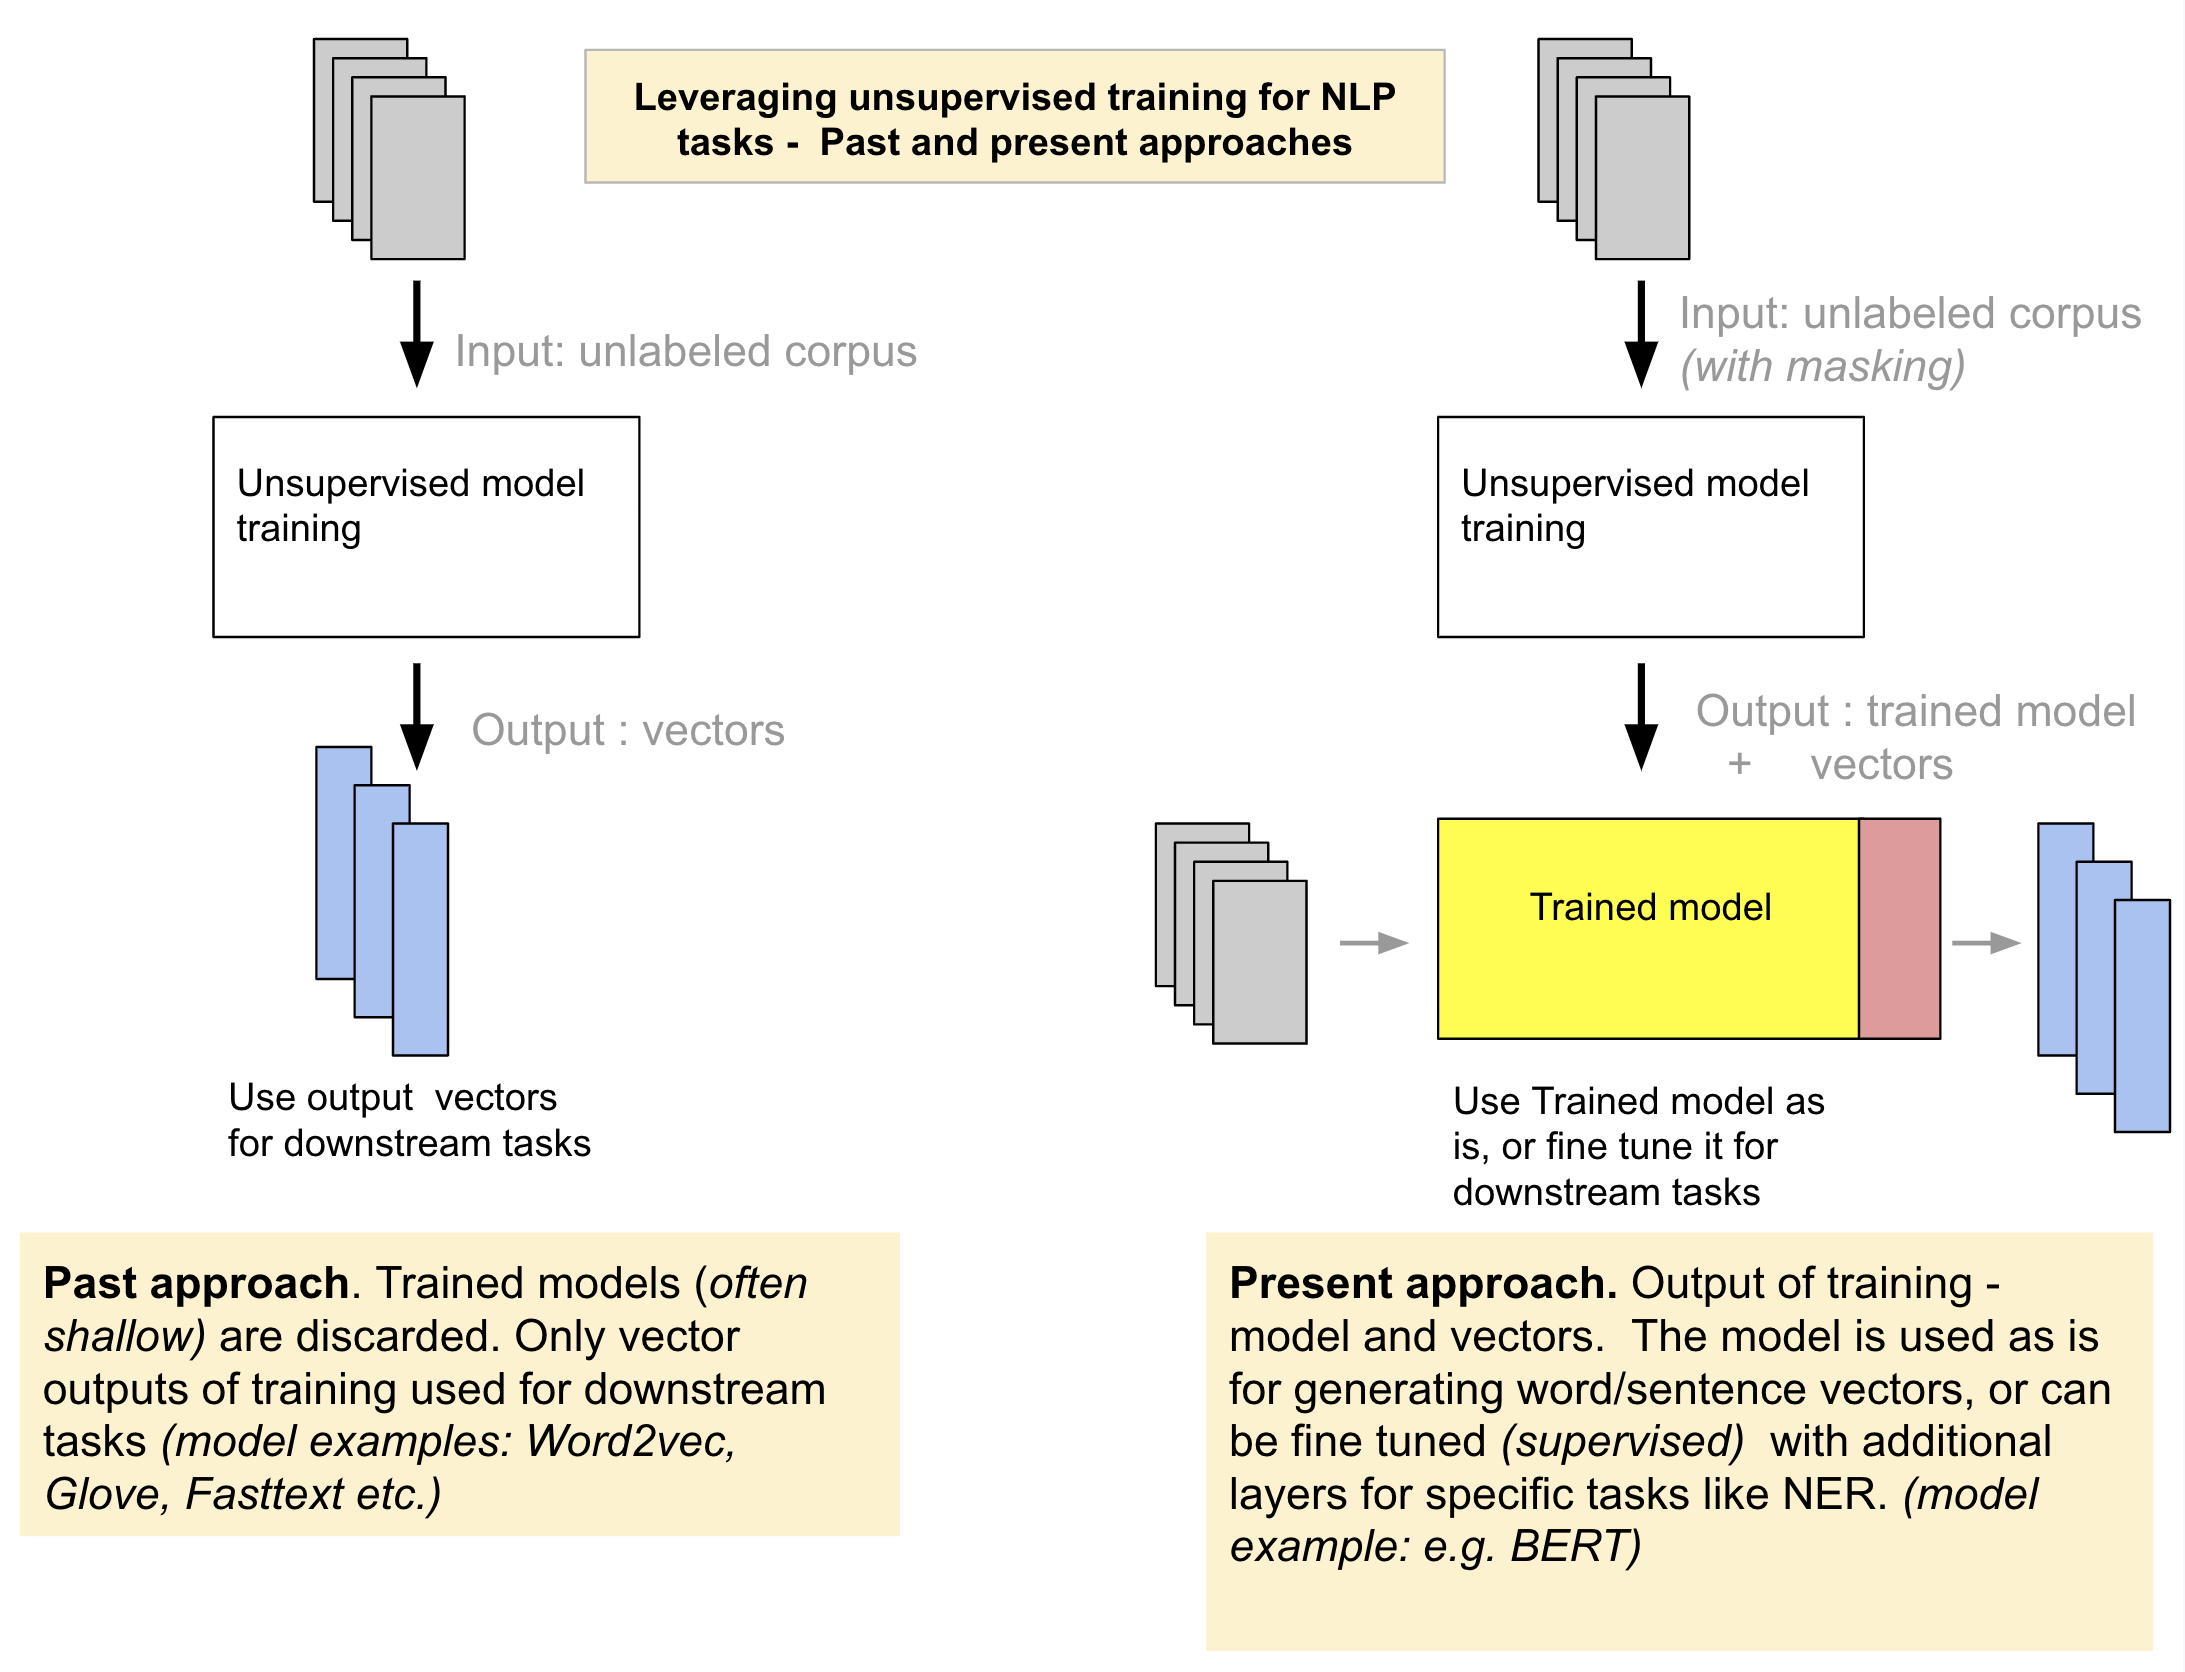
\includegraphics{img/difference_embeddings.png}

Die Grafik wurde von dieser
\href{https://www.quora.com/What-were-the-most-significant-Natural-Language-Processing-advances-in-2018/answer/Ajit-Rajasekharan}{Webseite}
entnommen.

    \hypertarget{elmo}{%
\subsection{ELMo}\label{elmo}}

\textbf{ELMo} (= Embeddings from Language Models) wurde Anfang 2018 von
Peters et. al.~veröffentlicht
(\href{https://arxiv.org/abs/1802.05365}{Paper}). Für das Training von
Embeddings verwendet ELMo ein \textbf{tiefes bidirektionales LSTM
Language Model}. Language Models werden dazu verwendet, anhand von
vorangegangen Wörtern das nächste Wort in einem Satz vorauszusagen. Dazu
müssen Language Models sowohl die semantischen als auch die
syntaktischen Eigenschaften von Wörtern kodieren, welches sie zu
geeignten Modellen für die Darstellung von Wörtern macht. Die
Bidirektionalität erlaubt es ELMo, nicht nur vorhergehende Wörter,
sondern auch nachfolgende Wörter für die Vorausage eines Wortes zu
verwenden. ELMo agiert beim Training nicht auf der Wortebene, sondern
verwendet ähnlich wie FastText Buchstabenvektoren, womit Wörter unter
Benutzung eines Lernmodells oder der Mittelwertsbildung der Wortvektoren
gebaut und das OOV-Problem umgangen werden kann. Trotzdem sind die
ausgegeben Vektoren letztendlich Wortvektoren und keine Buchstaben- oder
Teilwortvektoren.

Im Folgenden wird anhand eines Beispielsatzes die Funktionsweise der
ELMo-Embedding mithilfe der Bibliothek \textbf{Flair} demonstriert. Beim
Beispielsatz hat das Wort ``apple'' mehrere Bedeutungen, einmal ist das
Unternehmen gemeint und einmal die Frucht. Vergleicht man die beiden
Vektoren, erkennt man, dass diese durch unterschiedliche Vektoren
dargestellt werden. Anders als bei vorherigen Embedding-Verfahren wird
die Mehrdeutigkeit also dargestellt.

    \begin{tcolorbox}[breakable, size=fbox, boxrule=1pt, pad at break*=1mm,colback=cellbackground, colframe=cellborder]
\prompt{In}{incolor}{69}{\boxspacing}
\begin{Verbatim}[commandchars=\\\{\}]
\PY{n}{sentence5} \PY{o}{=} \PY{n}{Sentence}\PY{p}{(}\PY{l+s+s1}{\PYZsq{}}\PY{l+s+s1}{apple is a company but an apple is also a fruit}\PY{l+s+s1}{\PYZsq{}}\PY{p}{)}
\PY{n}{ELMoEmbeddings}\PY{p}{(}\PY{l+s+s2}{\PYZdq{}}\PY{l+s+s2}{original}\PY{l+s+s2}{\PYZdq{}}\PY{p}{)}\PY{o}{.}\PY{n}{embed}\PY{p}{(}\PY{n}{sentence5}\PY{p}{)}

\PY{n}{elmo\PYZus{}tensors} \PY{o}{=} \PY{p}{[}\PY{p}{]}

\PY{k}{for} \PY{n}{token} \PY{o+ow}{in} \PY{n}{sentence5}\PY{p}{:}
    \PY{k}{if} \PY{n}{token}\PY{o}{.}\PY{n}{text} \PY{o}{==} \PY{l+s+s2}{\PYZdq{}}\PY{l+s+s2}{apple}\PY{l+s+s2}{\PYZdq{}}\PY{p}{:}
        \PY{n}{elmo\PYZus{}tensors}\PY{o}{.}\PY{n}{append}\PY{p}{(}\PY{n}{token}\PY{o}{.}\PY{n}{embedding}\PY{p}{)}
    \PY{n+nb}{print}\PY{p}{(}\PY{l+s+sa}{f}\PY{l+s+s2}{\PYZdq{}}\PY{l+s+s2}{\PYZsq{}}\PY{l+s+si}{\PYZob{}}\PY{n}{token}\PY{o}{.}\PY{n}{text}\PY{l+s+si}{\PYZcb{}}\PY{l+s+s2}{\PYZsq{}}\PY{l+s+s2}{: }\PY{l+s+si}{\PYZob{}}\PY{n}{token}\PY{o}{.}\PY{n}{embedding}\PY{p}{[}\PY{p}{:}\PY{l+m+mi}{3}\PY{p}{]}\PY{l+s+si}{\PYZcb{}}\PY{l+s+s2}{ }\PY{l+s+s2}{\PYZdq{}} \PY{o}{+}
          \PY{l+s+sa}{f}\PY{l+s+s2}{\PYZdq{}}\PY{l+s+s2}{(Vektorlänge: }\PY{l+s+si}{\PYZob{}}\PY{n+nb}{len}\PY{p}{(}\PY{n}{token}\PY{o}{.}\PY{n}{embedding}\PY{p}{)}\PY{l+s+si}{\PYZcb{}}\PY{l+s+s2}{)}\PY{l+s+s2}{\PYZdq{}}\PY{p}{)}
\end{Verbatim}
\end{tcolorbox}

    \begin{Verbatim}[commandchars=\\\{\}]
'apple': tensor([0.1444, 0.0678, 0.3774]) (Vektorlänge: 3072)
'is': tensor([ 0.1915,  0.2300, -0.2894]) (Vektorlänge: 3072)
'a': tensor([ 0.1040,  0.1229, -0.0706]) (Vektorlänge: 3072)
'company': tensor([ 0.6496,  0.0804, -0.5390]) (Vektorlänge: 3072)
'but': tensor([-0.2404, -0.2742, -0.2190]) (Vektorlänge: 3072)
'an': tensor([ 0.0797,  0.1992, -0.0695]) (Vektorlänge: 3072)
'apple': tensor([0.1444, 0.0678, 0.3774]) (Vektorlänge: 3072)
'is': tensor([ 0.1915,  0.2300, -0.2894]) (Vektorlänge: 3072)
'also': tensor([ 0.8475, -0.2688,  0.2739]) (Vektorlänge: 3072)
'a': tensor([ 0.1040,  0.1229, -0.0706]) (Vektorlänge: 3072)
'fruit': tensor([-0.5279,  0.3975,  0.8766]) (Vektorlänge: 3072)
    \end{Verbatim}

    \begin{tcolorbox}[breakable, size=fbox, boxrule=1pt, pad at break*=1mm,colback=cellbackground, colframe=cellborder]
\prompt{In}{incolor}{70}{\boxspacing}
\begin{Verbatim}[commandchars=\\\{\}]
\PY{n}{diff} \PY{o}{=} \PY{n}{elmo\PYZus{}tensors}\PY{p}{[}\PY{l+m+mi}{1}\PY{p}{]} \PY{o}{\PYZhy{}} \PY{n}{elmo\PYZus{}tensors}\PY{p}{[}\PY{l+m+mi}{0}\PY{p}{]}
\PY{n+nb}{print}\PY{p}{(}\PY{l+s+s2}{\PYZdq{}}\PY{l+s+s2}{Die Vektoren der beiden unterschiedlichen Bedeutungen }\PY{l+s+s2}{\PYZdq{}} \PY{o}{+}
      \PY{l+s+s2}{\PYZdq{}}\PY{l+s+s2}{von }\PY{l+s+s2}{\PYZsq{}}\PY{l+s+s2}{apple}\PY{l+s+s2}{\PYZsq{}}\PY{l+s+s2}{ unterscheiden sich bei ELMo in }\PY{l+s+s2}{\PYZdq{}} \PY{o}{+}
      \PY{l+s+sa}{f}\PY{l+s+s2}{\PYZdq{}}\PY{l+s+si}{\PYZob{}}\PY{n+nb}{len}\PY{p}{(}\PY{p}{[}\PY{n}{i} \PY{k}{for} \PY{n}{i} \PY{o+ow}{in} \PY{n}{diff}\PY{o}{.}\PY{n}{tolist}\PY{p}{(}\PY{p}{)} \PY{k}{if} \PY{n}{i} \PY{o}{!=} \PY{l+m+mi}{0}\PY{p}{]}\PY{p}{)}\PY{l+s+si}{\PYZcb{}}\PY{l+s+s2}{ von 3072 Stellen.}\PY{l+s+s2}{\PYZdq{}}\PY{p}{)}
\end{Verbatim}
\end{tcolorbox}

    \begin{Verbatim}[commandchars=\\\{\}]
Die Vektoren der beiden unterschiedlichen Bedeutungen von 'apple' unterscheiden
sich bei ELMo in 2045 von 3072 Stellen.
    \end{Verbatim}

    \hypertarget{bert}{%
\subsection{BERT}\label{bert}}

\textbf{BERT} (= Bidirectional Encoder Representations from
Transformers) gehört wie \textbf{ELMo} zu den \textbf{contextualised
word embeddings} und wurde Ende 2018 von Devlin et. al.~veröffentlicht
(\href{https://arxiv.org/abs/1810.04805}{Paper}). BERT baut auf der
bidirektionalen Idee von ELMo auf, verwendet anstatt einem LSTM-Modell
jedoch ein \textbf{Transformers}-Modell um die Embeddings zu berechnen.
Beim Training verwendete BERT den sogenannten
\textbf{Attention}-Mechanismus des \textbf{Transformers}-Modell, der es
erlaubt, relevanten Worten in einer Sequenz mehr Bedeutung als anderen
Worten zuzuschreiben. Anders als vorhergehende Implementierungen des
Attention-Mechanismus verwendete BERT anstatt eines unidirektionalen
einen \textbf{bidirektionalen} Ansatz, bei dem nicht nur nachfolgende,
sondern auch vorhergehende Wörter betrachtet wurden. Der bidirektionale
Ansatz ist jedoch in dem Sinne problematisch, dass er Wörtern erlaubt,
sich indirekt ``selbst zu sehen'', wodurch das Modell in der Lage wäre,
das Zielwort relativ einfach vorauszusagen.

Zur Lösung dieses Problems benutzte BERT die Konzepte \textbf{Next
Sentence Prediction} und \textbf{Masked Language Modeling}. Bei der
\textbf{Next Sentence Prediction} (NSP) prüft BERT, ob ein nachfolgender
Satz kontextuell zum vorherigen Satz passt. Das \textbf{Masked Language
Modeling} (MLM) ist eine spezielle Form des Language Modelings. Dabei
werden zufällig 15\% der Wörter in jedem Satz der Trainingsdaten
ausgewählt, von denen wiederum 80\% durch ein spezielles
Maskierungstoken ausgetauscht, 10\% durch ein zufälliges Wort aus dem
Vokabular des Korpus ersetzt und 10\% der Wörter nicht verändert werden.
BERT versuchte dann im Training, die ausgewählten Tokens vorauszusagen,
wozu es die umliegenden, nicht maskierten Wörter verwendete. Dadurch
berücksichtigen die gelernten Gewichte anders als Word2Vec oder GloVe
den Kontext eines Wortes, was es BERT erlaubt, zwischen mehrdeutigen
Wörtern zu unterscheiden. Um das OOV-Problem zu umgehen, verwendete BERT
ähnlich wie FastText keine ganzen Wörter, sondern Teilwörter, mithilfe
derer verschiedene Wörter zusammengebaut werden können.

Im Folgenden wird anhand eines Beispielsatzes die Funktionsweise der
BERT-Embedding mithilfe der Bibliothek \textbf{Flair} demonstriert. Beim
Beispielsatz hat das Wort ``apple'' mehrere Bedeutungen, einmal ist das
Unternehmen gemeint und einmal die Frucht. Vergleicht man die beiden
Vektoren, erkennt man, dass diese durch unterschiedliche Vektoren
dargestellt werden. Anders als noch bei ELMo unterscheiden sich diese
Vektoren vollends voneinander, sie haben keine gemeinsamen Stellen.

    \begin{tcolorbox}[breakable, size=fbox, boxrule=1pt, pad at break*=1mm,colback=cellbackground, colframe=cellborder]
\prompt{In}{incolor}{49}{\boxspacing}
\begin{Verbatim}[commandchars=\\\{\}]
\PY{n}{sentence6} \PY{o}{=} \PY{n}{Sentence}\PY{p}{(}\PY{l+s+s1}{\PYZsq{}}\PY{l+s+s1}{apple is a company but an apple is also a fruit}\PY{l+s+s1}{\PYZsq{}}\PY{p}{)}
\PY{n}{BertEmbeddings}\PY{p}{(}\PY{p}{)}\PY{o}{.}\PY{n}{embed}\PY{p}{(}\PY{n}{sentence6}\PY{p}{)}

\PY{n}{bert\PYZus{}tensors} \PY{o}{=} \PY{p}{[}\PY{p}{]}

\PY{k}{for} \PY{n}{token} \PY{o+ow}{in} \PY{n}{sentence6}\PY{p}{:}
    \PY{k}{if} \PY{n}{token}\PY{o}{.}\PY{n}{text} \PY{o}{==} \PY{l+s+s2}{\PYZdq{}}\PY{l+s+s2}{apple}\PY{l+s+s2}{\PYZdq{}}\PY{p}{:}
        \PY{n}{bert\PYZus{}tensors}\PY{o}{.}\PY{n}{append}\PY{p}{(}\PY{n}{token}\PY{o}{.}\PY{n}{embedding}\PY{p}{)}
    \PY{n+nb}{print}\PY{p}{(}\PY{l+s+sa}{f}\PY{l+s+s2}{\PYZdq{}}\PY{l+s+s2}{\PYZsq{}}\PY{l+s+si}{\PYZob{}}\PY{n}{token}\PY{o}{.}\PY{n}{text}\PY{l+s+si}{\PYZcb{}}\PY{l+s+s2}{\PYZsq{}}\PY{l+s+s2}{: }\PY{l+s+si}{\PYZob{}}\PY{n}{token}\PY{o}{.}\PY{n}{embedding}\PY{p}{[}\PY{p}{:}\PY{l+m+mi}{3}\PY{p}{]}\PY{l+s+si}{\PYZcb{}}\PY{l+s+s2}{ }\PY{l+s+s2}{\PYZdq{}} \PY{o}{+}
          \PY{l+s+sa}{f}\PY{l+s+s2}{\PYZdq{}}\PY{l+s+s2}{(Vektorlänge: }\PY{l+s+si}{\PYZob{}}\PY{n+nb}{len}\PY{p}{(}\PY{n}{token}\PY{o}{.}\PY{n}{embedding}\PY{p}{)}\PY{l+s+si}{\PYZcb{}}\PY{l+s+s2}{)}\PY{l+s+s2}{\PYZdq{}}\PY{p}{)}
\end{Verbatim}
\end{tcolorbox}

    \begin{Verbatim}[commandchars=\\\{\}]
'apple': tensor([ 0.3007,  0.4433, -0.2990]) (Vektorlänge: 3072)
'is': tensor([-0.1345, -0.1533, -0.1418]) (Vektorlänge: 3072)
'a': tensor([-0.0250, -0.0645,  0.1348]) (Vektorlänge: 3072)
'company': tensor([ 0.2446, -0.1140,  0.0695]) (Vektorlänge: 3072)
'but': tensor([-0.2657, -0.2901,  0.1341]) (Vektorlänge: 3072)
'an': tensor([-0.1693,  1.0000, -0.0986]) (Vektorlänge: 3072)
'apple': tensor([ 0.0220,  0.8081, -0.1181]) (Vektorlänge: 3072)
'is': tensor([-0.3891,  0.3975,  0.1520]) (Vektorlänge: 3072)
'also': tensor([-0.7347, -0.0557, -0.2733]) (Vektorlänge: 3072)
'a': tensor([-0.1067,  0.3567,  0.2085]) (Vektorlänge: 3072)
'fruit': tensor([-0.1865,  0.4674, -0.2058]) (Vektorlänge: 3072)
    \end{Verbatim}

    \begin{tcolorbox}[breakable, size=fbox, boxrule=1pt, pad at break*=1mm,colback=cellbackground, colframe=cellborder]
\prompt{In}{incolor}{50}{\boxspacing}
\begin{Verbatim}[commandchars=\\\{\}]
\PY{n}{diff} \PY{o}{=} \PY{n}{bert\PYZus{}tensors}\PY{p}{[}\PY{l+m+mi}{1}\PY{p}{]} \PY{o}{\PYZhy{}} \PY{n}{bert\PYZus{}tensors}\PY{p}{[}\PY{l+m+mi}{0}\PY{p}{]}
\PY{n+nb}{print}\PY{p}{(}\PY{l+s+s2}{\PYZdq{}}\PY{l+s+s2}{Die Vektoren der beiden unterschiedlichen Bedeutungen }\PY{l+s+s2}{\PYZdq{}} \PY{o}{+}
      \PY{l+s+s2}{\PYZdq{}}\PY{l+s+s2}{von }\PY{l+s+s2}{\PYZsq{}}\PY{l+s+s2}{apple}\PY{l+s+s2}{\PYZsq{}}\PY{l+s+s2}{ unterscheiden sich bei BERT in }\PY{l+s+s2}{\PYZdq{}} \PY{o}{+}
      \PY{l+s+sa}{f}\PY{l+s+s2}{\PYZdq{}}\PY{l+s+si}{\PYZob{}}\PY{n+nb}{len}\PY{p}{(}\PY{p}{[}\PY{n}{i} \PY{k}{for} \PY{n}{i} \PY{o+ow}{in} \PY{n}{diff}\PY{o}{.}\PY{n}{tolist}\PY{p}{(}\PY{p}{)} \PY{k}{if} \PY{n}{i} \PY{o}{!=} \PY{l+m+mi}{0}\PY{p}{]}\PY{p}{)}\PY{l+s+si}{\PYZcb{}}\PY{l+s+s2}{ von 3072 Stellen.}\PY{l+s+s2}{\PYZdq{}}\PY{p}{)}
\end{Verbatim}
\end{tcolorbox}

    \begin{Verbatim}[commandchars=\\\{\}]
Die Vektoren der beiden unterschiedlichen Bedeutungen von 'apple' unterscheiden
sich bei BERT in 3072 von 3072 Stellen.
    \end{Verbatim}

    \begin{tcolorbox}[breakable, size=fbox, boxrule=1pt, pad at break*=1mm,colback=cellbackground, colframe=cellborder]
\prompt{In}{incolor}{ }{\boxspacing}
\begin{Verbatim}[commandchars=\\\{\}]

\end{Verbatim}
\end{tcolorbox}


    % Add a bibliography block to the postdoc
    
    
    
\end{document}
